% =====================================================================================
% Handcrafted, Learned, or Both? -- Capstone Final Report (Phases 1 and 2, IEEE conference format)
%
% COMPILED OUTPUT: report.pdf (same folder).
% TO RECOMPILE (Overleaf, pdfLaTeX): upload report.tex together with these 7 figures, copied from results/figures/:
%     eda_class_mean_images.png, results_pixels_vs_hog.png, cnn_training_curves.png, errors_confusion_cnn3_images.png,
%     errors_misclassified_rbf_svm_hog_shirt_vs_t-shirt_top.png, errors_misclassified_cnn3_images_shirt_vs_t-shirt_top.png,
%     hybrid_recall_vs_cnn3.png
%   IEEEtran, TikZ and pgfplots ship with Overleaf.
%
% Every number comes from results/summary_all.csv, results/metrics/*.json, results/training/*.csv, the saved test
% predictions and the outputs of notebooks 01-08. Confidence intervals (Wilson, 95%) and McNemar tests were computed
% from the saved predictions; no model was re-run on the test set.

% =====================================================================================
\documentclass[conference]{IEEEtran}
\IEEEoverridecommandlockouts

\usepackage[utf8]{inputenc}
\usepackage[T1]{fontenc}
\usepackage[final,expansion=false]{microtype}
\usepackage{graphicx}
\usepackage{booktabs}
\usepackage{multirow}
\usepackage{array}
\usepackage{amsmath,amssymb}
\usepackage{xcolor}
\usepackage{tikz}
\usetikzlibrary{positioning,arrows.meta,fit,backgrounds}
\usepackage{pgfplots}
\pgfplotsset{compat=1.18}
\usepackage{url}
\usepackage{cite}
\usepackage[hidelinks]{hyperref}
\usepackage[capitalise,nameinlink]{cleveref}

% ---- consistent notation -----------------------------------------------------------
\newcommand{\pp}{\,pp}                       % percentage points
\newcommand{\RQ}[1]{\textbf{RQ#1}}
\newcommand{\best}[1]{\textbf{#1}}
\newcommand{\arrowc}{\,$\rightarrow$\,}
\newcommand{\hyb}{\textsc{Hybrid}}           % RBF SVM on CNN3 features
\DeclareMathOperator*{\argmax}{arg\,max}

% ---- layout: no text in the margins, fewer half-empty float pages ---------------------
\setlength{\emergencystretch}{2em}
\renewcommand{\topfraction}{0.9}
\renewcommand{\bottomfraction}{0.6}
\renewcommand{\textfraction}{0.1}
\renewcommand{\floatpagefraction}{0.8}
\renewcommand{\dbltopfraction}{0.9}
\renewcommand{\dblfloatpagefraction}{0.8}
\setcounter{topnumber}{3}
\setcounter{dbltopnumber}{2}

\crefname{table}{Table}{Tables}
\crefname{figure}{Fig.}{Figs.}
\crefname{section}{Section}{Sections}
\crefname{equation}{Eq.}{Eqs.}

\begin{document}

\title{Handcrafted, Learned, or Both?\\[2pt]
\large A Leak-Free Study of Classical Pipelines, Small Convolutional Networks\\and Hybrid Features on Fashion-MNIST}

\author{
\IEEEauthorblockN{Tanmay Singh, Anand Mishra, Rajdeep Sanyal, Rajat Srivastav, Omved Nagre}
\IEEEauthorblockA{Newton School of Technology, Rishihood University\\
Advanced Machine Learning and Deep Learning --- Capstone Project (Phases 1 and 2)}
}

\maketitle

% =====================================================================================
\begin{abstract}
Deep networks are widely assumed to beat handcrafted image features, but how large the advantage is, where it comes
from, and what it costs are rarely measured under a protocol strict enough to trust. We answer these questions on
Fashion-MNIST with one fixed split, one evaluation function and a test set that is read exactly once per experiment and
logged. \emph{Phase~1} benchmarks five classical classifiers on raw pixels and on Histograms of Oriented Gradients (HOG):
the model selected on validation, an RBF support vector machine (SVM) on HOG, reaches 91.08\% test accuracy, and Shirt is
the hardest class for every model. \emph{Phase~2} tests two hypotheses stated before any network was trained: a small
convolutional neural network (CNN) beats 91.08\% (H1), and it does so chiefly by resolving the confusion among
upper-body garments (H2). A three-block CNN with 241{,}546 parameters reaches 92.09\% (95\% CI 91.54--92.60\%), 101 fewer
errors than the SVM (McNemar $p=2.2\times10^{-4}$), while predicting ${\sim}300\times$ faster from a model
${\sim}377\times$ smaller: H1 holds. H2 fails: Shirt recall is unchanged (75.1\% vs.\ 75.2\%), and the two models trade
shirts rather than fix them. Finally, a \emph{hybrid} that feeds the CNN's 128 learned features to the same RBF SVM
separates representation from classifier: it reaches 92.44\%, the best result in the study. Holding the classifier fixed,
learned features add 1.36 percentage points over HOG ($p=5.2\times10^{-7}$); holding the features fixed, the SVM adds
only 0.35 points over the CNN's own softmax layer ($p=0.012$). The gain is largely a property of the representation, and the
residual error---shared, with the same wrong label, by models that see the image in entirely different ways---appears
to be a property of the $28\times28$ data.
\end{abstract}

\begin{IEEEkeywords}
Fashion-MNIST, image classification, HOG, support vector machines, convolutional neural networks, learned features,
data leakage, McNemar test, error analysis
\end{IEEEkeywords}

% =====================================================================================
\section{Introduction}
\label{sec:intro}
An online clothing catalog that tags product photos automatically needs a classifier that is accurate, fast and small.
Convolutional networks are the usual answer for images, but whether they are \emph{necessary},
and \emph{why} they help, can only be judged against a strong, honestly evaluated classical baseline: one that never uses
the test set for a decision, trains every model on the same data, and reports uncertainty and paired tests rather than
single accuracy numbers.

Fashion-MNIST~\cite{xiao2017fashion} was released as a harder drop-in replacement for MNIST, together with a benchmark of
classical classifiers on raw pixels whose best entry, an RBF support vector machine, reached 89.7\%. Our Phase~1
study~\cite{phase1report} revisited that classical baseline under a leak-free protocol, added handcrafted gradient
features, and raised it to 91.08\%, but found that no classical model recognizes shirts reliably. On the deep-learning
side, Agarap~\cite{agarap2017cnnsvm} replaced the softmax output of a small CNN with an SVM and found it slightly
\emph{worse} on Fashion-MNIST (90.72\% vs.\ 91.86\%). Together these results leave a question open. A CNN differs from a
kernel machine on handcrafted features in two ways at once---it \emph{learns} its features, and it \emph{decides} with a
different classifier---so when it wins, which of the two is responsible? Comparisons that change both components at once
cannot say.

\textbf{Problem statement.} Given the 70{,}000 grayscale $28\times28$ images of Fashion-MNIST~\cite{xiao2017fashion} in ten
garment classes, we ask (a)~how far fixed, handcrafted representations go; (b)~whether a small learned representation
goes further, and on which classes; and (c)~whether any improvement comes from the learned \emph{features} or from the
\emph{classifier} trained with them---all under a single protocol in which every choice is made on validation data and
the test set is touched once per experiment. The study ran in two phases:
\begin{itemize}
  \item \textbf{Phase~1 (classical,~\cite{phase1report}).} \RQ{1}: How accurate is classical ML on raw pixels? \RQ{2}: Do HOG features beat
        pixels, and for which models? \RQ{3}: Which model gives the best accuracy--speed--size trade-off? \RQ{4}: Which
        classes are confused, and why do handcrafted features fail there?
  \item \textbf{Phase~2 (deep).} \RQ{5}: Does a small CNN beat the best classical model? \RQ{6}: Does it reduce the
        upper-body garment confusion? \RQ{7}: Does a third convolutional block help? \RQ{8}: What does the CNN cost?
        \RQ{9}: Does an RBF SVM on the CNN's learned features beat the CNN's own classifier---that is, is the gain in the
        representation or in the classifier?
\end{itemize}
Phase~1 closed with two falsifiable hypotheses, recorded before any network existed:
\textbf{H1}---a small CNN trained under the same protocol exceeds 91.08\% test accuracy; and \textbf{H2}---its gain comes
\emph{chiefly} from resolving confusions within \{T-shirt/top, Pullover, Coat, Shirt\}, because learned local filters
capture the collars, buttons and cuffs that fixed edge histograms miss. The protocol of the hybrid experiment (RQ9) was
likewise fixed and committed before it was run.

\textbf{Contributions.}
\begin{enumerate}
  \item A reproducible benchmark of \textbf{15 experiments}---12 classical, 2 CNNs, 1 hybrid---sharing one committed
        split, one evaluation function and a test-set audit log with exactly one entry per experiment.
  \item A validation-only selection protocol, including a correction for models tuned on different amounts of data,
        and a cost analysis that counts feature-extraction time rather than model time alone.
  \item A controlled test of a pre-registered mechanism (H2) with paired significance tests and image-level agreement
        analysis, showing that the CNN's gain is real but does not arise where predicted.
  \item A \emph{feature--classifier decomposition}: by moving one component at a time between the best classical
        model and the CNN, we attribute most of the deep-learning gain to the representation, and we reconcile this
        with the earlier CNN--SVM result on the same dataset~\cite{agarap2017cnnsvm}.
  \item Evidence that the residual error is dominated by images that independent models misclassify identically, a
        ceiling that neither representation crosses.
\end{enumerate}

\textbf{Summary of findings.} The best classical pipeline reaches 91.08\%. CNN3 reaches 92.09\% and is two orders of
magnitude cheaper (H1 supported), but Shirt recall does not move (H2 rejected). The hybrid reaches 92.44\%; learned
features account for most of the improvement, the classifier for a small, validation-invisible remainder.
\Cref{tab:headline} summarizes the three representative models.

\textbf{Organization.} \Cref{sec:related} positions the study against the three works it builds on.
\Cref{sec:background} fixes notation and the statistical tools; \cref{sec:protocol} describes the shared protocol.
\Cref{sec:phase1,sec:phase2,sec:hybrid} follow the study in the order it was run---classical pipelines, CNNs, and the
hybrid that separates features from classifier---and \cref{sec:discussion,sec:conclusion} interpret the results and
their limits.

\begin{table}[t]
  \centering
  \caption{Headline Results on the 10{,}000-Image Test Set}
  \label{tab:headline}
  \setlength{\tabcolsep}{4pt}
  \resizebox{\columnwidth}{!}{%
  \begin{tabular}{@{}l c c c r r@{}}
    \toprule
    Model & Test acc.\ (95\% CI) & Macro-F1 & Shirt & ms/1k & Size \\
    \midrule
    RBF SVM / HOG  & 91.08 (90.51--91.62) & 0.9108 & 75.2 & 29{,}093 & 366\,MB \\
    CNN3           & 92.09 (91.54--92.60) & 0.9208 & 75.1 & \best{94} & \best{0.97\,MB} \\
    \hyb{}         & \best{92.44} (91.91--92.94) & \best{0.9241} & 73.8 & 609 & 9.7\,MB \\
    \bottomrule
  \end{tabular}}\\[2pt]
  {\footnotesize Shirt: recall (\%). ms/1k: end-to-end prediction time per 1{,}000 images, including feature extraction.}
\end{table}

% =====================================================================================
\section{Related Work and Positioning}
\label{sec:related}
The study builds on three lines of evidence, one per reference, and is designed to answer the question they leave open.

\textbf{The benchmark.} Xiao et al.~\cite{xiao2017fashion} built Fashion-MNIST to keep MNIST's format---70{,}000
grayscale $28\times28$ images, ten balanced classes, a fixed 60k/10k split---while removing its ceiling: classifiers that
are nearly perfect on digits fall well below that on garments. Their benchmark of scikit-learn classifiers on raw pixels,
led by an RBF SVM at 89.7\%, is the natural reference for classical pixel pipelines. It reports test accuracy across
grids of settings, without a separate validation split or confidence intervals, which is appropriate for introducing a
dataset but not for deciding whether one model is better than another.

\textbf{The classical baseline.} Our Phase~1 study~\cite{phase1report} supplied that missing discipline. It fixed a
stratified validation split, moved every choice onto it, read the test set once per experiment through a logged
function, and compared five classifiers on raw pixels and on Histograms of Oriented Gradients (HOG). Its pixel RBF SVM
reproduces the benchmark's 89.7\%; HOG raises the best model to 91.08\%. Its error analysis found Shirt to be the
hardest class for every model and the four upper-body garments to account for most errors, and it closed with two
falsifiable hypotheses about what a CNN would change (\cref{sec:intro}). The present paper inherits its split,
evaluation code and audit log unchanged, so every number reported here is directly comparable with it.

\textbf{CNN features and SVM classifiers.} Agarap~\cite{agarap2017cnnsvm} asked whether an SVM is a better output layer
than softmax for a CNN. A two-convolutional-layer network was trained end to end on MNIST and Fashion-MNIST with either
a softmax or a linear SVM objective on top; on Fashion-MNIST the SVM variant scored 90.72\% against 91.86\% for softmax.
Because the SVM is trained \emph{jointly} with the network, the two variants end up with different features as well as
different classifiers, and the SVM is linear, so it cannot draw the curved boundaries a kernel provides. The result
therefore shows that replacing the softmax does not automatically help; it does not say how much of a CNN's advantage
lies in its features.

\textbf{This paper.} We close that gap with a controlled design. The CNN is trained once and then \emph{frozen}, and its
features are passed to the same RBF SVM, with the same grid and protocol, that Phase~1 used on HOG. Each comparison then
changes exactly one component, so the effect of learned features and the effect of the classifier can be measured
separately, on the same split and with paired significance tests (\cref{sec:hybrid}).

% =====================================================================================
\section{Problem Formulation and Background}
\label{sec:background}

\subsection{Task and Metrics}
Let $\mathcal{D}=\{(\mathbf{x}_n,y_n)\}$ with $\mathbf{x}_n\in[0,1]^{28\times28}$ and $y_n\in\{1,\dots,K\}$, $K=10$.
A classifier is the composition $f=h\circ\phi$ of a representation $\phi$ (pixels, HOG or learned) and a decision rule
$h$. On the test set of $n=10{,}000$ images we report accuracy $\hat p$, per-class precision $P_k$ and recall $R_k$, and
macro-F1,
\begin{equation}
  \mathrm{F1}_{\text{macro}} = \frac{1}{K}\sum_{k=1}^{K}\frac{2P_kR_k}{P_k+R_k},
  \label{eq:f1}
\end{equation}
which weights a weak class as heavily as a strong one. Uncertainty in accuracy is given by the Wilson score
interval with $z=1.96$,
\begin{equation}
  \frac{\hat p+\frac{z^2}{2n}\pm z\sqrt{\frac{\hat p(1-\hat p)}{n}+\frac{z^2}{4n^2}}}{1+\frac{z^2}{n}},
  \label{eq:wilson}
\end{equation}
about $\pm0.55$\pp{} wide at 91\% accuracy. Two classifiers $A$ and $B$ are compared on the \emph{same} test images with
McNemar's test. If $b$ images are classified correctly only by $A$ and
$c$ only by $B$, then under the null hypothesis of equal error rates
\begin{equation}
  \chi^2=\frac{(|b-c|-1)^2}{b+c}\;\sim\;\chi^2_1 ,
  \label{eq:mcnemar}
\end{equation}
with continuity correction. Images both models get right or both get wrong carry no information about which is
better. In every case reported, the exact binomial $p$-value leads to the same conclusion as the $\chi^2$
approximation.

\subsection{Classical Representations and Classifiers}
\textbf{HOG.} The image is divided into cells of $c\times c$ pixels; each cell receives a histogram of $o$ gradient
orientations weighted by gradient magnitude, and overlapping blocks of $b\times b$ cells are normalized together
(L2-Hys), which makes the descriptor robust to contrast. For a $28\times28$ image the descriptor length is
\begin{equation}
  d = \left(\tfrac{28}{c}-b+1\right)^{2} b^{2}\, o .
  \label{eq:hogdim}
\end{equation}

\textbf{Classifiers.} \emph{Logistic Regression} minimizes cross-entropy with an L2 penalty of strength $1/C$.
\emph{$k$-NN} labels an image by its $k$ nearest training images. A \emph{Random Forest} averages decision trees grown on
bootstrap samples with random feature subsets. \emph{Linear} and \emph{kernel SVMs} find a maximum-margin boundary; the
kernel variant uses
\begin{equation}
  K(\mathbf{x},\mathbf{x}') = \exp\!\left(-\gamma\,\lVert\mathbf{x}-\mathbf{x}'\rVert^2\right),
  \label{eq:rbf}
\end{equation}
and decides each one-vs-one binary problem by
\begin{equation}
  h(\mathbf{x})=\operatorname{sign}\Big(\sum_{i\in\mathcal{S}}\alpha_i y_i K(\mathbf{x}_i,\mathbf{x})+\beta\Big),
  \label{eq:svm}
\end{equation}
so its cost is proportional to the number of support vectors $|\mathcal{S}|$ times the
feature dimension. scikit-learn's default bandwidth $\gamma=\texttt{scale}$ is $1/(d\cdot\operatorname{Var}[\mathbf{X}])$.
All classical models use scikit-learn, HOG uses scikit-image, and the CNNs are built in PyTorch.

\subsection{Convolutional Networks}
\textbf{Convolution.} A layer with $F$ filters of size $k\times k$ over $C$ input channels computes
\begin{equation}
  z_{f,i,j} = b_f + \sum_{c=1}^{C}\sum_{u=1}^{k}\sum_{v=1}^{k} w_{f,c,u,v}\; x_{c,\,i+u-1,\,j+v-1},
  \label{eq:conv}
\end{equation}
followed by the ReLU $a=\max(0,z)$. Local connectivity and weight sharing make the layer
translation-equivariant with only $(k^2C+1)F$ parameters. A $2\times2$ max-pooling layer keeps the largest activation per
window, halving the resolution and adding tolerance to small shifts.

\textbf{Loss and optimization.} The network outputs scores $s_1,\dots,s_K$ and is trained to minimize the mini-batch
cross-entropy
\begin{equation}
  \mathcal{L}(\theta) = -\frac{1}{|\mathcal{B}|}\sum_{n\in\mathcal{B}} \log \frac{e^{s_{y_n}(\mathbf{x}_n)}}{\sum_{k=1}^{K} e^{s_k(\mathbf{x}_n)}},
  \label{eq:ce}
\end{equation}
the objective of multinomial logistic regression, now optimized jointly with the features. With gradient
$\mathbf{g}_t=\nabla_\theta\mathcal{L}$ computed by backpropagation, Adam
updates
\begin{equation}
  \begin{aligned}
    \mathbf{m}_t &= \beta_1\mathbf{m}_{t-1}+(1-\beta_1)\,\mathbf{g}_t,\\
    \mathbf{v}_t &= \beta_2\mathbf{v}_{t-1}+(1-\beta_2)\,\mathbf{g}_t^{2},\\
    \hat{\mathbf{m}}_t &= \frac{\mathbf{m}_t}{1-\beta_1^t},\quad
    \hat{\mathbf{v}}_t = \frac{\mathbf{v}_t}{1-\beta_2^t},
  \end{aligned}
  \label{eq:adam}
\end{equation}
and $\theta_t=\theta_{t-1}-\eta\,\hat{\mathbf{m}}_t/(\sqrt{\hat{\mathbf{v}}_t}+\epsilon)$, with $\beta_1=0.9$,
$\beta_2=0.999$, $\epsilon=10^{-8}$.

\textbf{Regularization.} During training, dropout multiplies the penultimate activations by
a mask $m_i\sim\mathrm{Bernoulli}(1-p)$ and rescales by $1/(1-p)$, so no rescaling is needed at test time, when dropout
is off. Early stopping keeps the weights with the lowest validation loss and stops after a fixed
number of epochs (the \emph{patience}) without improvement.

% =====================================================================================
\section{Data and Experimental Protocol}
\label{sec:protocol}

\textbf{Data.} Fashion-MNIST has 60{,}000 training and 10{,}000 test images in ten balanced classes: T-shirt/top,
Trouser, Pullover, Dress, Coat, Sandal, Shirt, Sneaker, Bag and Ankle boot. The four official files are verified against
their published MD5 checksums; automated checks confirm shapes, labels, exactly 6{,}000 training and 1{,}000 test images
per class, and no exact duplicates within or across splits.

\textbf{Fixed split.} A stratified validation set of 6{,}000 images (600 per class, seed 42) is carved from the
training set, leaving 54{,}000 training images. The validation indices are committed (MD5
\texttt{54ff6b78\allowbreak b27109cd\allowbreak fc3ebe72\allowbreak 04040a07}), so every experiment in both phases uses
an identical split. Pixels are scaled to $[0,1]$; no statistic is computed from validation or test data.

\textbf{Leakage controls.}
(i)~The test set is read only inside two functions, \texttt{final\_test\_run()} and \texttt{final\_test\_run\_cnn()},
once per experiment; every call appends a row to an audit log, which ends with exactly \textbf{15 rows}, one per
experiment. (ii)~Every choice---hyperparameters, HOG settings, network depth, final model---is made on validation.
(iii)~Feature scaling lives inside scikit-learn pipelines, so it is fitted only on the rows a model trains on, including
inside cross-validation folds. (iv)~Exploratory analysis uses the training split only. (v)~CNNs update their weights on
the training split only; validation is used for early stopping and selection, under \texttt{torch.no\_grad()}.
(vi)~All error analysis reads predictions saved at test time; no model predicts on the test set twice.

\textbf{Procedure.} \Cref{fig:protocol} shows the three tracks. Classical models fit each grid point on 54k images, are
selected on validation, refit on all 60k training-plus-validation images and tested once. CNNs train on 54k with early
stopping on validation and are not refit, because validation is consumed by early stopping; they therefore learn from
10\% less data than the classical models, a handicap that can only understate their advantage. The hybrid reuses the
classical track on features produced by the frozen, already-trained CNN. Each test evaluation records accuracy,
macro-F1, per-class precision and recall, the confusion matrix, training time, model-only prediction time per 1{,}000
images (best of three runs) and model size (bytes of the serialized model).

\begin{figure}[t]
\centering
\resizebox{\linewidth}{!}{%
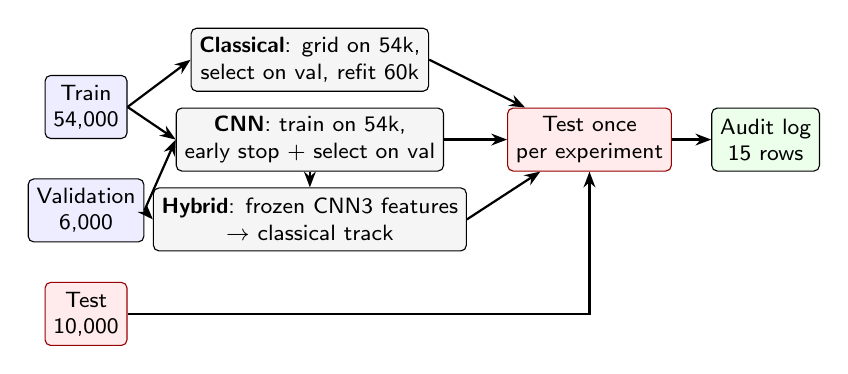
\begin{tikzpicture}[
  font=\sffamily\footnotesize,
  box/.style={draw, rounded corners=2pt, align=center, minimum height=8mm, inner sep=3pt},
  data/.style={box, fill=blue!7},
  proc/.style={box, fill=gray!8},
  lock/.style={box, fill=red!8, draw=red!60!black},
  arr/.style={-{Stealth[length=2mm]}, thick}
]
  \node[data] (tr)  {Train\\54{,}000};
  \node[data, below=5mm of tr] (va) {Validation\\6{,}000};
  \node[lock, below=5mm of va] (te) {Test\\10{,}000};

  \node[proc, right=8mm of tr, yshift=6mm] (cl) {\textbf{Classical}: grid on 54k,\\select on val, refit 60k};
  \node[proc, below=2mm of cl] (cn) {\textbf{CNN}: train on 54k,\\early stop + select on val};
  \node[proc, below=2mm of cn] (hy) {\textbf{Hybrid}: frozen CNN3 features\\$\to$ classical track};

  \node[lock, right=8mm of cn] (once) {Test once\\per experiment};
  \node[box, right=5mm of once, fill=green!8] (log) {Audit log\\15 rows};

  \draw[arr] (tr.east) -- (cl.west);
  \draw[arr] (tr.east) -- (cn.west);
  \draw[arr] (va.east) -- (cn.west);
  \draw[arr] (va.east) -- (hy.west);
  \draw[arr] (cn.south) -- (hy.north);
  \draw[arr] (cl.east) -- (once);
  \draw[arr] (cn.east) -- (once);
  \draw[arr] (hy.east) -- (once);
  \draw[arr] (te.east) -| (once.south);
  \draw[arr] (once) -- (log);
\end{tikzpicture}}
\caption{Evaluation protocol shared by all 15 experiments. Every decision is taken on validation; the test set (red) is
read once per experiment, after all choices are fixed, and each read is logged.}
\label{fig:protocol}
\end{figure}

\textbf{Exploratory analysis.} Pixels are highly redundant: PCA needs 84 of 784 components to keep 90\% of the variance.
The class-mean images of the upper-body garments are nearly identical (\cref{fig:eda}; cosine similarity 0.987 for
Coat--Shirt, 0.984 for Pullover--Coat, 0.983 for Pullover--Shirt), and in a t-SNE map
Pullover, Coat and Shirt form one mixed cloud. Before training any model we therefore predicted that Shirt would have
the lowest recall and that most errors would fall within the upper-body group.

\begin{figure}[t]
  \centering
  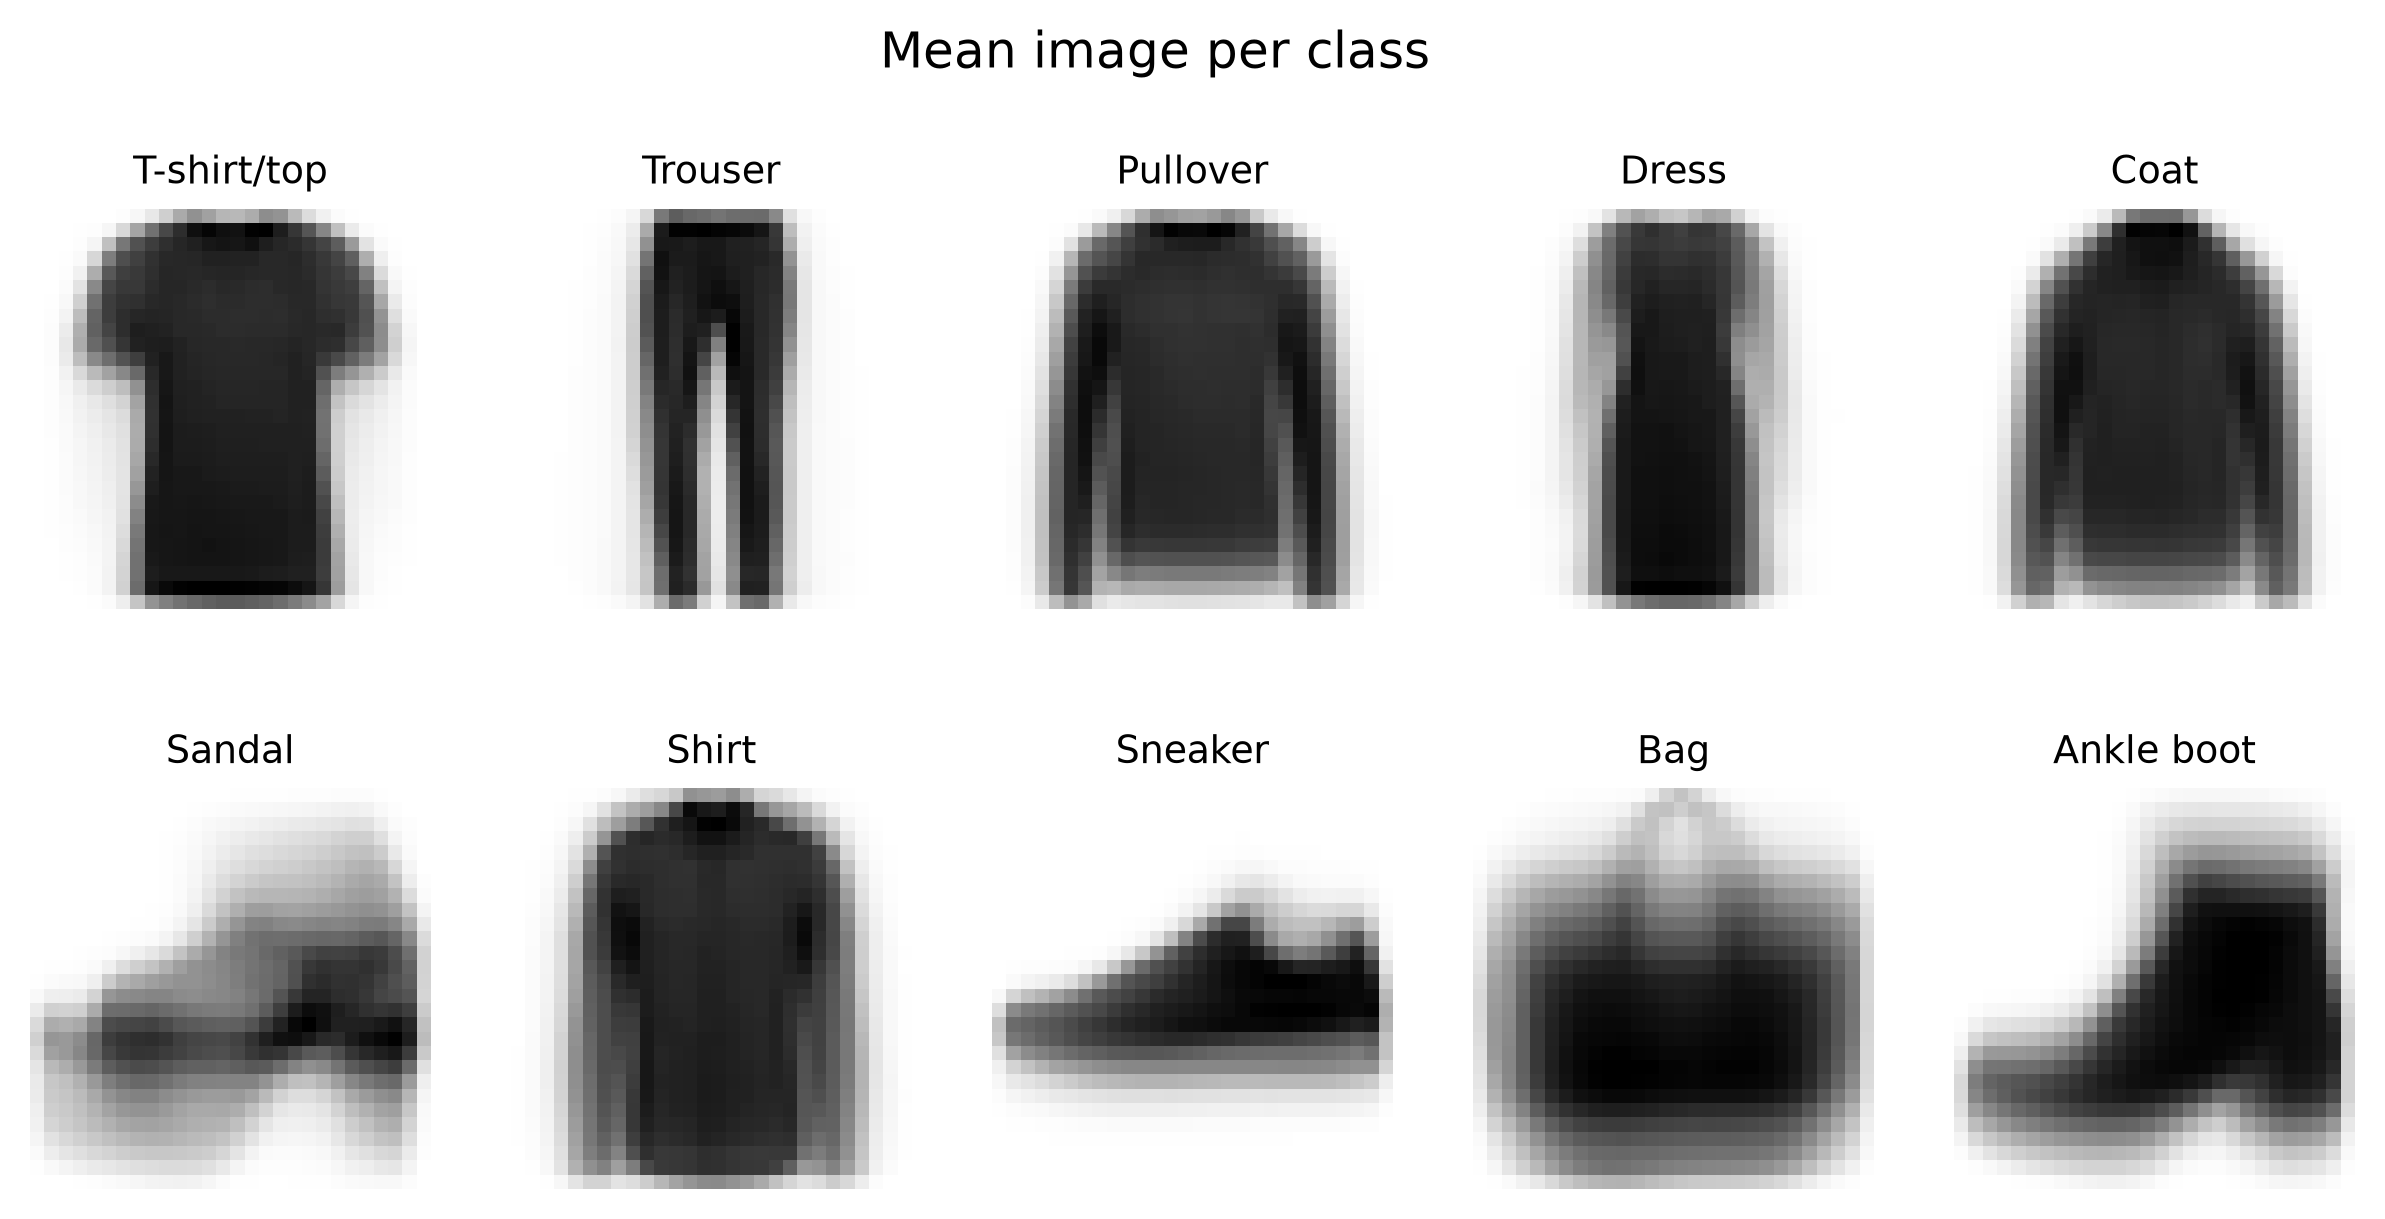
\includegraphics[width=\linewidth]{eda_class_mean_images.png}
  \caption{Mean training image of each class. The four upper-body garments are nearly indistinguishable on average.}
  \label{fig:eda}
\end{figure}

% =====================================================================================
\section{Phase 1: Classical Pipelines}
\label{sec:phase1}
This section summarizes the Phase~1 study~\cite{phase1report}: the classical results that Phase~2 must beat, and the
error pattern that motivated its hypotheses.

\subsection{Representations and Tuning}
\textbf{Pixels} are the flattened 784-dimensional image; flattening discards which pixels are neighbors. \textbf{HOG}
was configured by a sweep of $3\times2\times2=12$ settings ($o\in\{6,9,12\}$, $c\in\{4,7\}$, $b\in\{1,2\}$), each scored on
validation with a fast proxy (a linear SVM trained by SGD). Small cells win by 4--8\pp{} and block normalization adds
2--3\pp; the selected setting, $o=12$, $c=4$, $b=2$, gives $d=1{,}728$ by \cref{eq:hogdim} (proxy validation 0.8818) and
costs about 216\,ms per 1{,}000 images to extract.

\Cref{tab:grids} lists the validation grids. Kernel-SVM training scales super-linearly with the number of samples, so the
RBF SVM's grid was searched on a stratified 10{,}000-image subset. Its tuning-time validation scores therefore came from
far less data than every other model's; \emph{before} choosing the final model, the selected RBF settings were refit on
the full 54k training split and scored on the same validation set, with no new search and no test data. On this equal
footing the validation ranking is RBF SVM\,/\,HOG (0.9157) $>$ RBF SVM\,/\,pixels (0.9082) $>$ Logistic
Regression\,/\,HOG (0.8927).

\begin{table}[t]
  \centering
  \caption{Phase 1 Validation Grids and Selected Settings}
  \label{tab:grids}
  \setlength{\tabcolsep}{3pt}
  \renewcommand{\arraystretch}{1.1}
  \begin{tabular}{@{}>{\raggedright\arraybackslash}p{1.3cm} >{\raggedright\arraybackslash}p{3.2cm} >{\raggedright\arraybackslash}p{3.0cm}@{}}
    \toprule
    Model & Grid & Selected (pixels / HOG) \\
    \midrule
    Log.\ Reg. & $C\in\{0.01,0.1,1,10\}$ & $C=0.01$ / $C=0.01$ \\
    $k$-NN & $k\in\{1,3,5,7,9\}$; uniform / distance; Euclidean / Manhattan
           & $k{=}3$, distance, Manhattan / $k{=}3$, distance, Euclidean \\
    Rand.\ Forest & trees $\{100,300\}$; depth $\{\text{None},20,40\}$; features $\{\sqrt{p},\log_2 p\}$
           & 300, depth 20, $\sqrt{p}$ / 300, full depth, $\sqrt{p}$ \\
    Linear SVM & $C\in\{0.01,0.1,1\}$ & $C=0.01$ / $C=0.01$ \\
    RBF SVM & $C\in\{0.1,1,10\}$; $\gamma\in\{\text{scale},0.01,0.001\}$ (10k subset)
           & $C{=}10,\gamma{=}0.001$ / $C{=}10,\gamma{=}\text{scale}$ \\
    \bottomrule
  \end{tabular}
\end{table}

\subsection{Results (RQ1--RQ3)}
\Cref{tab:results} reports all experiments of both phases. \textbf{RQ1:} the best pixel model is the RBF SVM at 89.70\%,
matching the best pixel model of the original benchmark~\cite{xiao2017fashion}; the linear models reach only 83.78--84.72\%,
because a single pixel records brightness at one location and a linear boundary in pixel space cannot express shape.
\textbf{RQ2:} HOG helps linear models most---$+5.20$\pp{} for the Linear SVM and $+4.14$\pp{} for Logistic
Regression---and lifts the RBF SVM by $+1.38$\pp{} to 91.08\% (\cref{fig:pixhog}). It does not help Random Forest
($-0.53$\pp) or $k$-NN ($+0.20$\pp, inside the interval). On paired predictions the HOG SVM fixes 515 images the pixel
SVM gets wrong and breaks 377 ($\chi^2=21.0$, $p=4.5\times10^{-6}$), so the gain is significant. A 5-fold
cross-validation of the selected model on a 10k subset gives $0.8775\pm0.0054$, indicating a stable configuration.

\textbf{RQ3:} counting HOG extraction, three classical options stand out: Random Forest on pixels (87.56\% in about
12\,ms per 1{,}000 images, but a 366\,MB model), Linear SVM on HOG (88.98\% from a 181\,KB model in about 219\,ms) and
the RBF SVM on HOG (91.08\% in up to 29\,s, because every prediction is compared with 26{,}343 support vectors). $k$-NN is
slower and less accurate than the forest and is never the right choice. \Cref{fig:pareto} places these against the
Phase~2 models.

\begin{figure}[t]
  \centering
  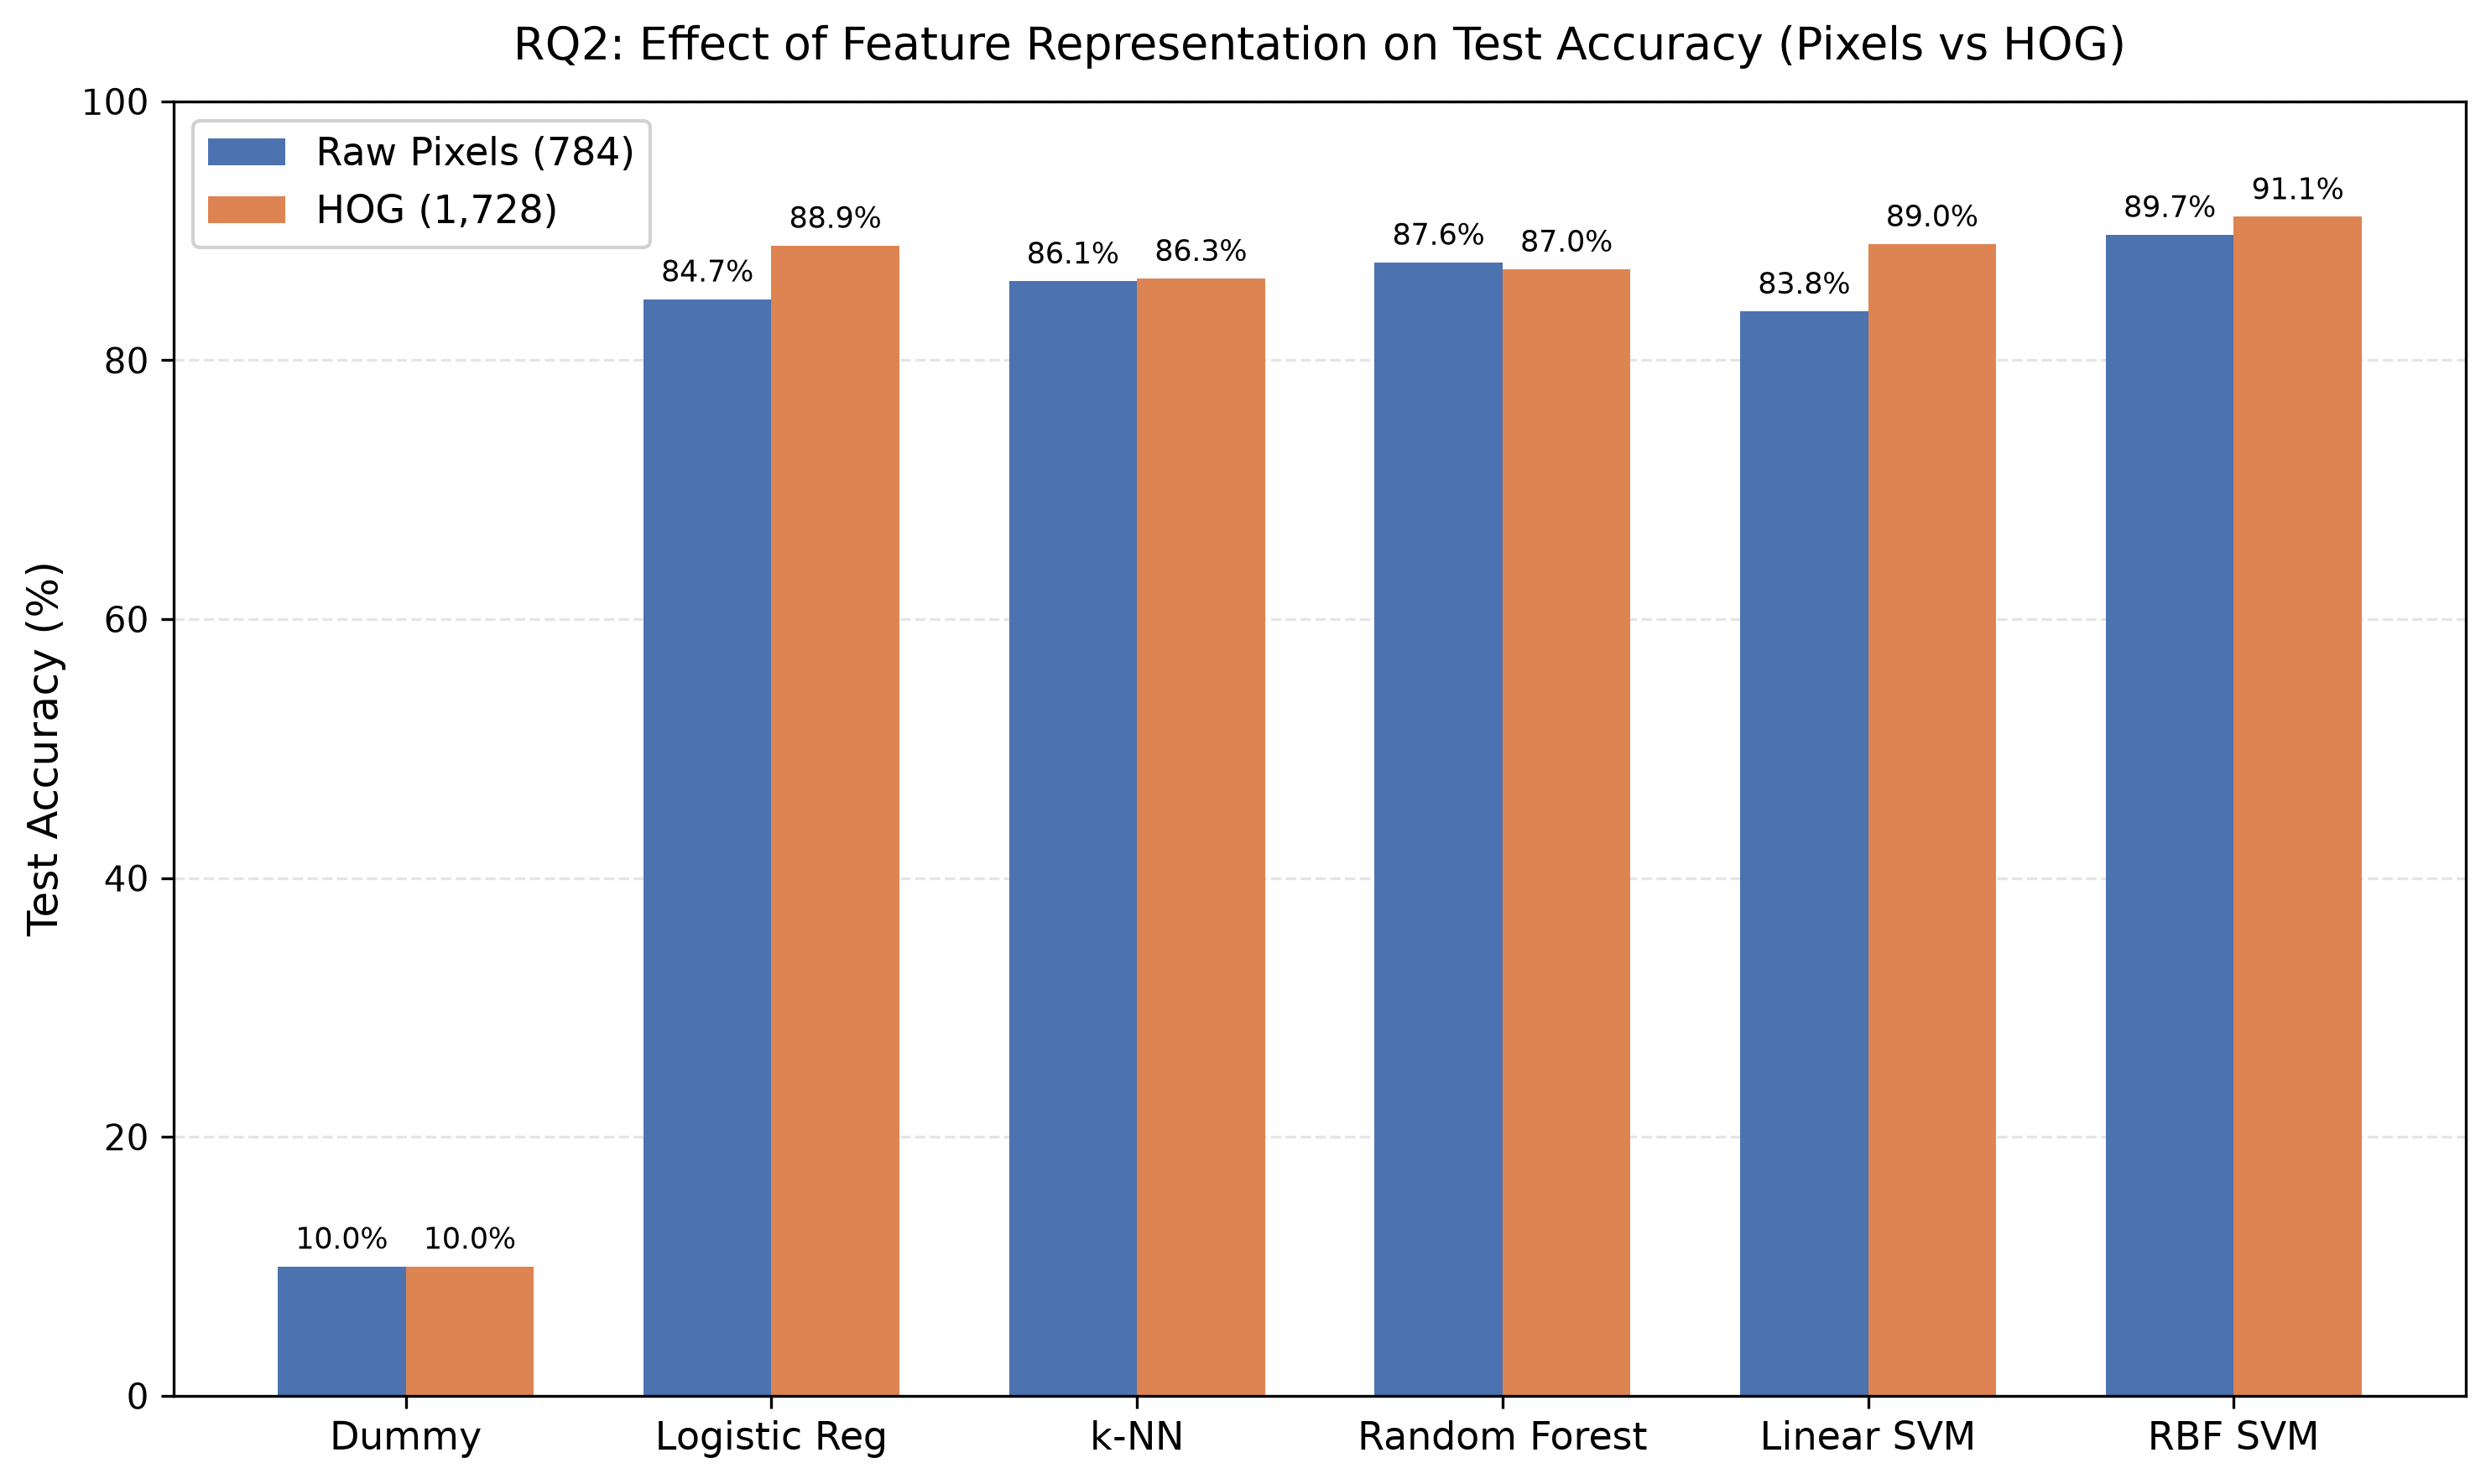
\includegraphics[width=0.92\linewidth]{results_pixels_vs_hog.png}
  \caption{Test accuracy of each classical model on pixels vs.\ HOG (RQ2). HOG transforms the linear models but does not
  help trees or nearest neighbors.}
  \label{fig:pixhog}
\end{figure}

\begin{table*}[t]
  \centering
  \caption{All 15 Experiments: Same Split, Same Evaluation Code, One Test Run Each}
  \label{tab:results}
  \setlength{\tabcolsep}{4pt}
  \resizebox{\textwidth}{!}{%
  \begin{tabular}{@{}l l c c c c r r r r@{}}
    \toprule
    Model & Representation & Val.\ acc. & Test acc. & 95\% CI (\%) & Macro-F1 & Errors & Train (s) & Pred.\ (ms/1k) & Size \\
    \midrule
    \multicolumn{10}{@{}l}{\emph{Phase 1: classical pipelines}} \\
    \multirow{2}{*}{Majority class} & Pixels & 0.1000 & 0.1000 & 9.43--10.60 & 0.0182 & 9{,}000 & 0.00 & 0.00$^{\mathrm{a}}$ & 709\,B \\
                                    & HOG    & 0.1000 & 0.1000 & 9.43--10.60 & 0.0182 & 9{,}000 & 0.16 & 0.01$^{\mathrm{a}}$ & 709\,B \\
    \multirow{2}{*}{Logistic Regression} & Pixels & 0.8642 & 0.8472 & 84.00--85.41 & 0.8464 & 1{,}528 & n/a$^{\mathrm{b}}$ & n/a$^{\mathrm{b}}$ & 51.4\,KB \\
                                         & HOG    & 0.8927 & 0.8886 & 88.23--89.46 & 0.8885 & 1{,}114 & n/a$^{\mathrm{b}}$ & n/a$^{\mathrm{b}}$ & 111.8\,KB \\
    \multirow{2}{*}{$k$-NN} & Pixels & 0.8747 & 0.8611 & 85.42--86.77 & 0.8614 & 1{,}389 & 0.49 & 6{,}926.61 & 188.7\,MB \\
                            & HOG    & 0.8728 & 0.8631 & 85.62--86.97 & 0.8623 & 1{,}369 & 1.29 & 731.13 & 415.2\,MB \\
    \multirow{2}{*}{Random Forest} & Pixels & 0.8867 & 0.8756 & 86.90--88.19 & 0.8741 & 1{,}244 & 32.83 & 12.16 & 366.5\,MB \\
                                   & HOG    & 0.8735 & 0.8703 & 86.36--87.67 & 0.8692 & 1{,}297 & 68.53 & 19.02 & 500.7\,MB \\
    \multirow{2}{*}{Linear SVM} & Pixels & 0.8583 & 0.8378 & 83.04--84.49 & 0.8353 & 1{,}622 & 99.24 & 1.22 & 82.7\,KB \\
                                & HOG    & 0.8900 & 0.8898 & 88.35--89.58 & 0.8892 & 1{,}102 & 162.04 & 2.62 & 180.8\,KB \\
    \multirow{2}{*}{RBF SVM} & Pixels & 0.9082 & 0.8970 & 89.09--90.28 & 0.8967 & 1{,}030 & 195.67 & 4{,}766.94 & 125.1\,MB \\
                             & HOG    & 0.9157 & 0.9108 & 90.51--91.62 & 0.9108 & 892 & 451.43 & 28{,}876.96$^{\mathrm{c}}$ & 366.2\,MB \\
    \midrule
    \multicolumn{10}{@{}l}{\emph{Phase 2: convolutional networks (trained on 54k, not refit)}} \\
    CNN2 & Image & 0.9228 & 0.9185 & 91.30--92.37 & 0.9176 & 815 & 198.22 & 58.36 & 1.69\,MB \\
    CNN3 & Image & 0.9308 & 0.9209 & 91.54--92.60 & 0.9208 & 791 & 416.13 & 94.43 & 0.97\,MB \\
    \midrule
    \multicolumn{10}{@{}l}{\emph{Phase 2: hybrid}} \\
    \best{RBF SVM} & \best{CNN3 features} & \best{0.9313} & \best{0.9244} & \best{91.91--92.94} & \best{0.9241} & \best{756} & 7.36$^{\mathrm{d}}$ & 491.23$^{\mathrm{d}}$ & 8.7\,MB$^{\mathrm{d}}$ \\
    \bottomrule
  \end{tabular}}\\[3pt]
  \begin{minipage}{\textwidth}\footnotesize
    Val.\ acc.: model trained on 54k (RBF SVMs refit on 54k for comparability). Test: classical and hybrid models
          refit on 60k; CNNs trained on 54k. CI: Wilson 95\% interval, \cref{eq:wilson}. Pred.: model-only time per
          1{,}000 test images, best of three; HOG extraction adds $\approx$216\,ms. Size: serialized model. Best result
          in bold.\\
    $^{\mathrm{a}}$\,Measured on a different machine; excluded from speed comparisons.\\
    $^{\mathrm{b}}$\,Not comparable (runs overlapped other workloads); accuracy unaffected.\\
    $^{\mathrm{c}}$\,26{,}343 support vectors; treated as an upper bound.\\
    $^{\mathrm{d}}$\,SVM only: 7{,}919 support vectors on precomputed features. CNN3 feature extraction adds $\approx$118\,ms per
          1{,}000 images, the CNN3 layers $\approx$0.97\,MB, and training CNN3 once 416\,s.\\
    Timing hardware: $k$-NN, CNNs and hybrid on an Apple M3; Random Forest and RBF/Linear SVMs on an Apple M3 Pro;
          4 threads throughout.
  \end{minipage}
\end{table*}

\subsection{Error Analysis (RQ4)}
Shirt has the lowest recall of the ten classes for \emph{every} trained classical model, from 50.9\% (Linear SVM, pixels)
to 75.2\% (RBF SVM, HOG), and confusions within \{T-shirt/top, Pullover, Coat, Shirt\} make up 56--66\% of every model's
errors. The selected model's largest confusions are Shirt\arrowc T-shirt/top (104), T-shirt/top\arrowc Shirt (91) and
Pullover\arrowc Shirt (66). Both outcomes match the predictions made from the data before training. The two best
classical models share 515 errors, 391 of them with the same wrong label---a first sign that part of the residual error
lies in the images rather than in the representation. At $28\times28$, the collar and buttons that distinguish a shirt
occupy a handful of pixels, poorly captured by fixed edge histograms; Phase~2 tests whether learned filters do better.

% =====================================================================================
\section{Phase 2: Small Convolutional Networks}
\label{sec:phase2}

\subsection{Architectures}
\label{sec:cnn-arch}
Both networks stack \emph{conv blocks}---a $3\times3$ convolution with padding~1, a ReLU and $2\times2$ max
pooling---followed by a dense classifier (\cref{fig:arch,tab:arch}). CNN2 uses blocks of 32 and 64 filters; CNN3 adds a
third block of 128 filters. The third pooling layer shrinks the map from $7\times7$ to $3\times3$, so the input to the
first dense layer falls from 3{,}136 to 1{,}152 values and the deeper network has 43\% \emph{fewer} parameters, while
needing 79\% more multiply--accumulate operations (MACs), because the added convolution runs at every position of a
$7\times7$ map. Stacking enlarges the receptive field from $10\times10$ to $22\times22$ pixels---most of the garment.

\begin{figure}[t]
\centering
\resizebox{\linewidth}{!}{%
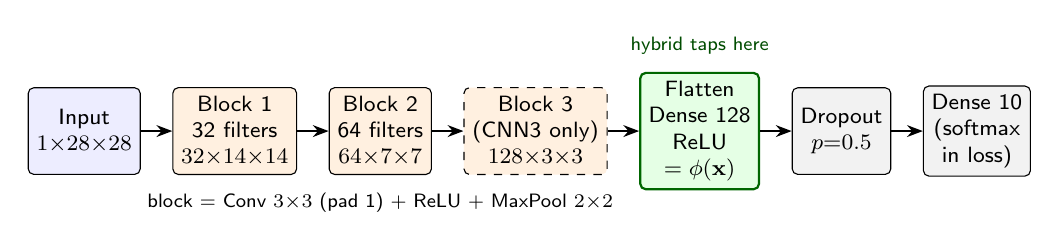
\begin{tikzpicture}[
  font=\sffamily\footnotesize,
  blk/.style={draw, rounded corners=2pt, align=center, minimum height=11mm, inner sep=3pt},
  inp/.style={blk, fill=blue!7},
  conv/.style={blk, fill=orange!12},
  dense/.style={blk, fill=gray!10},
  extra/.style={blk, fill=orange!12, dashed},
  feat/.style={blk, fill=green!10, draw=green!40!black, thick},
  arr/.style={-{Stealth[length=2mm]}, thick}
]
  \node[inp] (in) {Input\\$1{\times}28{\times}28$};
  \node[conv, right=4mm of in] (b1) {Block 1\\32 filters\\$32{\times}14{\times}14$};
  \node[conv, right=4mm of b1] (b2) {Block 2\\64 filters\\$64{\times}7{\times}7$};
  \node[extra, right=4mm of b2] (b3) {Block 3\\(CNN3 only)\\$128{\times}3{\times}3$};
  \node[feat, right=4mm of b3] (fc) {Flatten\\Dense 128\\ReLU\\$=\phi(\mathbf{x})$};
  \node[dense, right=4mm of fc] (do) {Dropout\\$p{=}0.5$};
  \node[dense, right=4mm of do] (out) {Dense 10\\(softmax\\in loss)};
  \draw[arr] (in) -- (b1); \draw[arr] (b1) -- (b2); \draw[arr] (b2) -- (b3);
  \draw[arr] (b3) -- (fc); \draw[arr] (fc) -- (do); \draw[arr] (do) -- (out);
  \node[below=1mm of b2, font=\sffamily\scriptsize, align=center] {block = Conv $3{\times}3$ (pad 1) + ReLU + MaxPool $2{\times}2$};
  \node[above=1mm of fc, font=\sffamily\scriptsize, align=center, text=green!30!black] {hybrid taps here};
\end{tikzpicture}}
\caption{Architecture. CNN2 skips the dashed block and flattens $64{\times}7{\times}7=3{,}136$ values; CNN3 flattens
$128{\times}3{\times}3=1{,}152$. The 128 activations after the first dense layer (green) are the learned features used by
the hybrid (\cref{sec:hybrid}).}
\label{fig:arch}
\end{figure}

\begin{table}[t]
  \centering
  \caption{Parameters, Compute and Receptive Field}
  \label{tab:arch}
  \setlength{\tabcolsep}{4pt}
  \resizebox{\columnwidth}{!}{%
  \begin{tabular}{@{}l r r r@{}}
    \toprule
    Layer & CNN2 params & CNN3 params & MACs per image \\
    \midrule
    Conv 1 ($1\to32$)   & 320       & 320       & 225{,}792 \\
    Conv 2 ($32\to64$)  & 18{,}496  & 18{,}496  & 3{,}612{,}672 \\
    Conv 3 ($64\to128$) & ---       & 73{,}856  & 3{,}612{,}672 (CNN3) \\
    Dense ($\to128$)    & 401{,}536 & 147{,}584 & 401{,}408 / 147{,}456 \\
    Dense ($128\to10$)  & 1{,}290   & 1{,}290   & 1{,}280 \\
    \midrule
    \textbf{Total}      & \textbf{421{,}642} & \textbf{241{,}546} & \textbf{4.24M / 7.60M} \\
    Receptive field     & $10\times10$ & $22\times22$ & \\
    \bottomrule
  \end{tabular}}
\end{table}

\subsection{Training and Model Selection (RQ7)}
\label{sec:cnn-train}
Both networks use identical, untuned settings: cross-entropy (\cref{eq:ce}), Adam (\cref{eq:adam}) with $\eta=10^{-3}$,
mini-batches of 64 (844 updates per epoch), at most 30 epochs, early stopping on validation loss with patience~5 and the
best weights restored, and dropout $p=0.5$. Training is deterministic: all generators are seeded with 42, deterministic
kernels are enforced, and the training function creates its own starting weights and data loaders, so a fresh-process
retraining reproduces every reported validation statistic exactly. Training runs on an Apple M3 CPU with four threads,
the thread count used for the classical models.

\Cref{fig:curves} shows both runs. Validation loss bottoms out at epoch~9 for CNN2 and epoch~12 for CNN3; afterwards
training loss keeps falling (CNN3: 0.175\arrowc0.127) while validation loss rises (0.193\arrowc0.208), the signature of
overfitting, and early stopping ends each run five epochs later. At the selected epoch, training accuracy (measured with
dropout on) is within 0.5\pp{} of validation accuracy.

\begin{figure}[t]
  \centering
  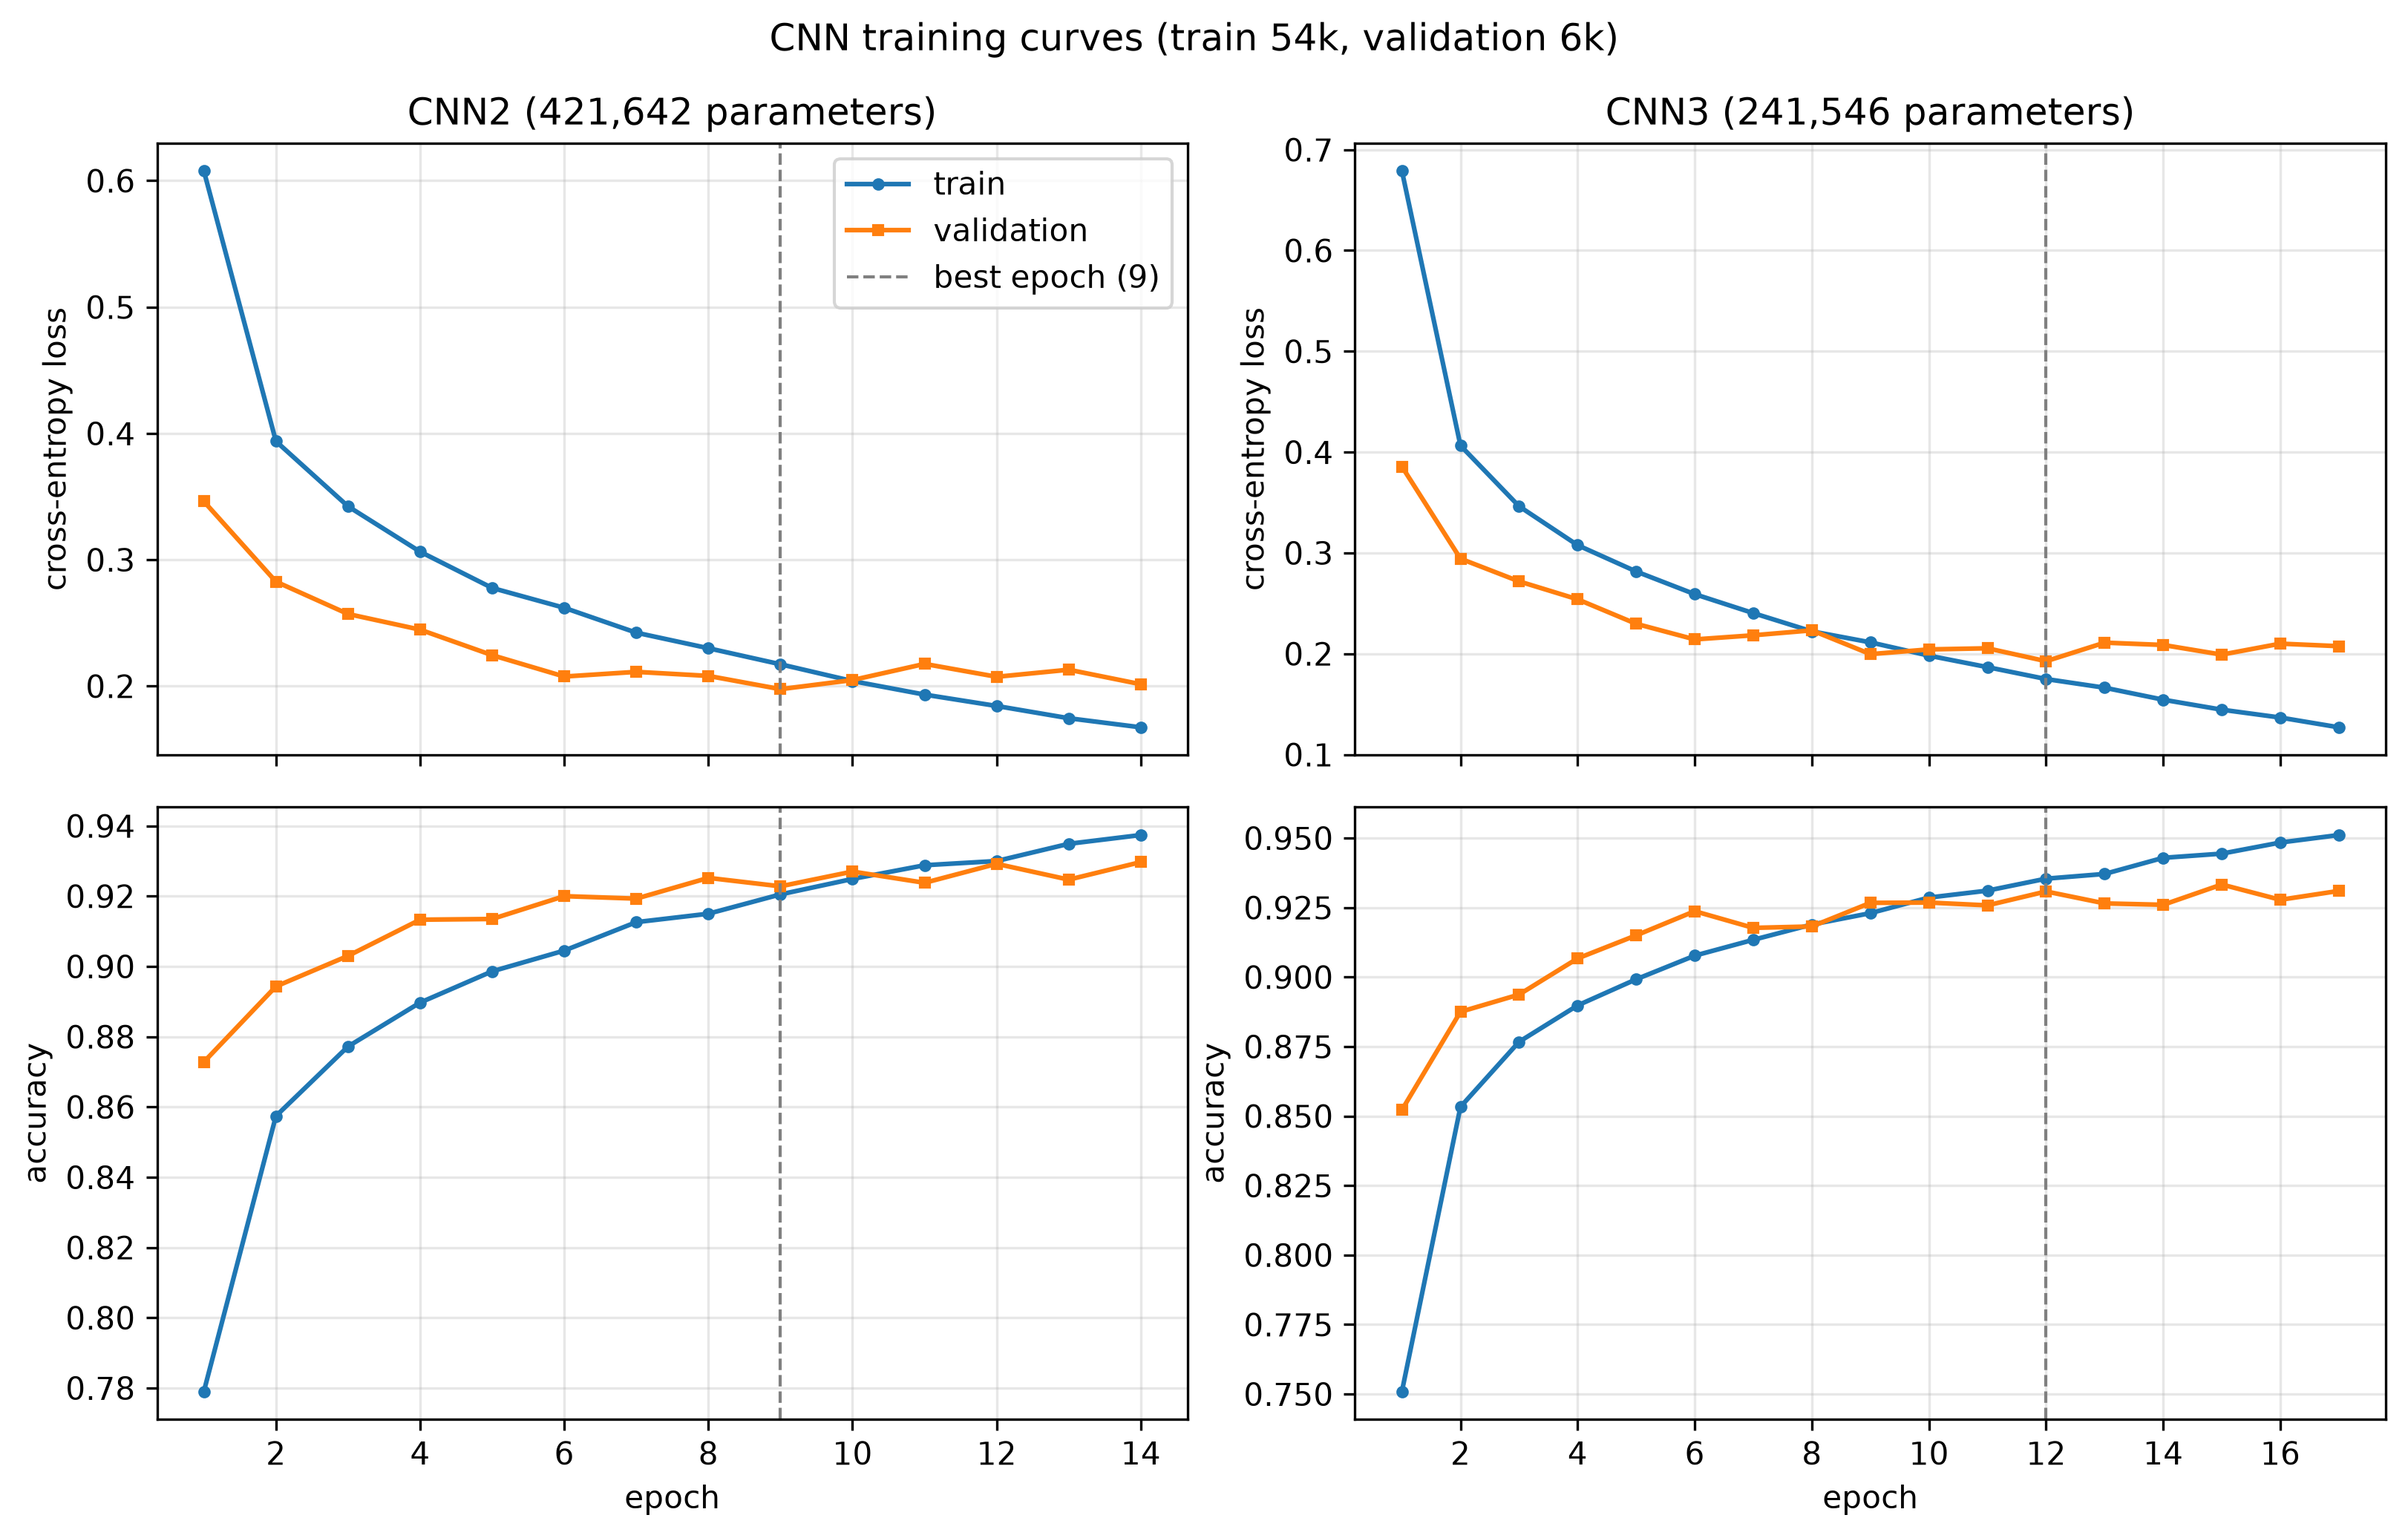
\includegraphics[width=\linewidth]{cnn_training_curves.png}
  \caption{Training and validation loss (top) and accuracy (bottom) per epoch. Dashed lines mark the epoch with the
  lowest validation loss, whose weights are kept.}
  \label{fig:curves}
\end{figure}

The selection rule, fixed before training, was \emph{higher validation accuracy, ties to fewer parameters}: CNN2 scored
0.9228 (best epoch 9 of 14, 198\,s) and CNN3 \textbf{0.9308} (12 of 17, 416\,s), so \textbf{CNN3 is selected}; both exceed
the best classical validation score (0.9157). We do not read the 0.8\pp{} gap as evidence that depth helps: a preliminary
CNN2 run differing only in mini-batch order reached 0.9320, and on the test set the two networks disagree on 506 images
with an almost even split (265 vs.\ 241; $\chi^2=1.05$, $p=0.31$). What depth demonstrably buys is a 43\% smaller model.

\subsection{Test Performance and Cost (RQ5, RQ8)}
\label{sec:cnn-test}
CNN3 reaches \textbf{92.09\%} test accuracy and \textbf{0.9208} macro-F1 (\cref{tab:results}); CNN2 reaches 91.85\% and
0.9176. Against the RBF SVM on HOG, CNN3 corrects 417 images and breaks 316 (\cref{tab:agree}), a net 101:
$\chi^2=13.6$, $p=2.2\times10^{-4}$. CNN2's advantage is also significant (407 vs.\ 330, $p=5.1\times10^{-3}$).
\textbf{H1 is supported.}

The CNN is also far cheaper. CNN3 classifies 1{,}000 images in 94\,ms against ${\approx}29.1$\,s end to end for the SVM,
a ${\sim}300\times$ speed-up, from a 0.97\,MB model ${\sim}377\times$ smaller than the SVM's 366\,MB of support vectors.
The SVM's cost grows with its training set; the CNN's is fixed by its architecture. Within the CNNs, prediction time
tracks MACs rather than parameters: CNN3 is 43\% smaller but 62\% slower than CNN2. \Cref{fig:pareto} shows that both
networks are more accurate \emph{and} faster end to end than every classical model except the two cheapest pixel models,
the Random Forest (12\,ms) and the Linear SVM (1.2\,ms), which are faster but 4.3\pp{} and 8.1\pp{} less accurate than CNN2.

\begin{figure}[t]
  \centering
  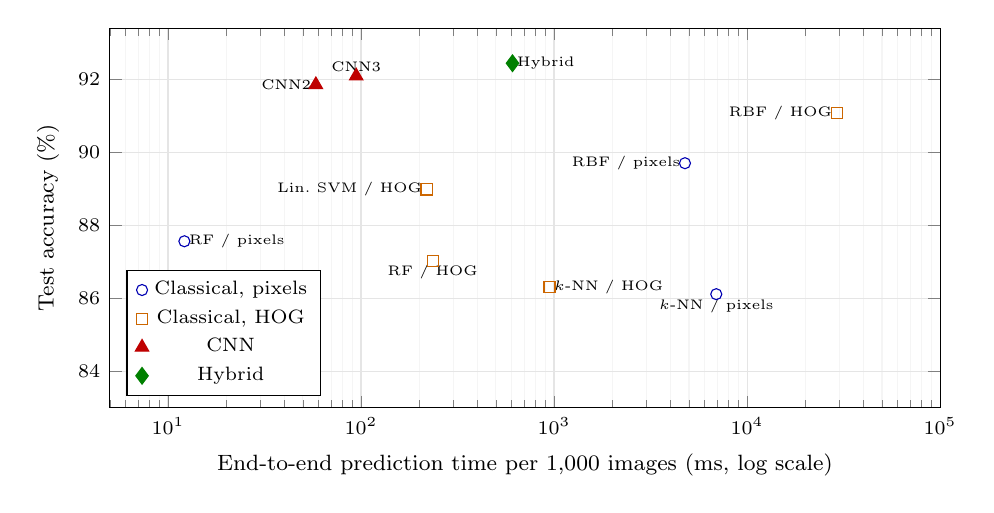
\begin{tikzpicture}[lbl/.style={font=\tiny, inner sep=1.5pt}]
    \begin{semilogxaxis}[
      width=\linewidth, height=6.4cm,
      xlabel={End-to-end prediction time per 1{,}000 images (ms, log scale)},
      ylabel={Test accuracy (\%)},
      xmin=5, xmax=100000, ymin=83, ymax=93.4,
      grid=both, grid style={gray!20}, minor grid style={gray!8},
      tick label style={font=\scriptsize}, label style={font=\footnotesize},
      legend style={font=\scriptsize, at={(0.02,0.03)}, anchor=south west},
    ]
      \addplot[only marks, mark=o, mark size=2pt, blue!70!black] coordinates {
        (12.16,87.56) (6926.61,86.11) (4766.94,89.70)};
      \addlegendentry{Classical, pixels}
      \addplot[only marks, mark=square, mark size=2pt, orange!80!black] coordinates {
        (235.02,87.03) (947.13,86.31) (218.62,88.98) (29092.96,91.08)};
      \addlegendentry{Classical, HOG}
      \addplot[only marks, mark=triangle*, mark size=2.8pt, red!75!black] coordinates {
        (58.36,91.85) (94.43,92.09)};
      \addlegendentry{CNN}
      \addplot[only marks, mark=diamond*, mark size=3pt, green!50!black] coordinates {
        (609.23,92.44)};
      \addlegendentry{Hybrid}
      \node[lbl, anchor=west]  at (axis cs:12.16,87.56)    {RF / pixels};
      \node[lbl, anchor=north] at (axis cs:6926.61,86.11)  {$k$-NN / pixels};
      \node[lbl, anchor=east]  at (axis cs:4766.94,89.70)  {RBF / pixels};
      \node[lbl, anchor=north] at (axis cs:235.02,87.03)   {RF / HOG};
      \node[lbl, anchor=west]  at (axis cs:947.13,86.31)   {$k$-NN / HOG};
      \node[lbl, anchor=east]  at (axis cs:218.62,88.98)   {Lin.\ SVM / HOG};
      \node[lbl, anchor=east]  at (axis cs:29092.96,91.08) {RBF / HOG};
      \node[lbl, anchor=east]  at (axis cs:58.36,91.85)    {CNN2};
      \node[lbl, anchor=south] at (axis cs:94.43,92.09)    {CNN3};
      \node[lbl, anchor=west]  at (axis cs:609.23,92.44)   {Hybrid};
    \end{semilogxaxis}
  \end{tikzpicture}
  \caption{Accuracy vs.\ end-to-end prediction time (feature extraction included). The CNNs sit alone in the
  upper-left corner; the hybrid buys 0.35\pp{} over CNN3 for ${\sim}6.5\times$ the time. Linear SVM on pixels (1.2\,ms,
  83.78\%) lies left of the axis; Logistic Regression timings are not comparable and are omitted.}
  \label{fig:pareto}
\end{figure}

\subsection{Error Analysis (RQ6)}
\label{sec:cnn-errors}
Relative to the SVM, CNN3 reduces errors on T-shirt/top ($-22$), Pullover ($-28$), Coat ($-15$), Trouser ($-14$),
Sneaker ($-14$) and Sandal ($-12$), and is slightly worse on Dress ($+8$). On \textbf{Shirt it changes nothing}: recall
is 75.1\% vs.\ 75.2\%, and Shirt\arrowc T-shirt/top remains the largest confusion (110 vs.\ 104; \cref{fig:cm}). CNN3
labels fewer non-shirts as Shirt (precision 77.4\% vs.\ 75.3\%) but finds no more of the real ones. Of the 1{,}000 test
shirts, 661 are classified correctly by both models, 90 only by CNN3, 91 only by the SVM and 158 by neither (McNemar
$p=1.0$): the models \emph{trade} shirts. Because the CNN removes easier errors first, the four upper-body classes hold a
\emph{larger} share of what remains: 539 of 791 errors (68.1\%) against 573 of 892 (64.2\%). \textbf{H2 is rejected.}

\begin{figure}[t]
  \centering
  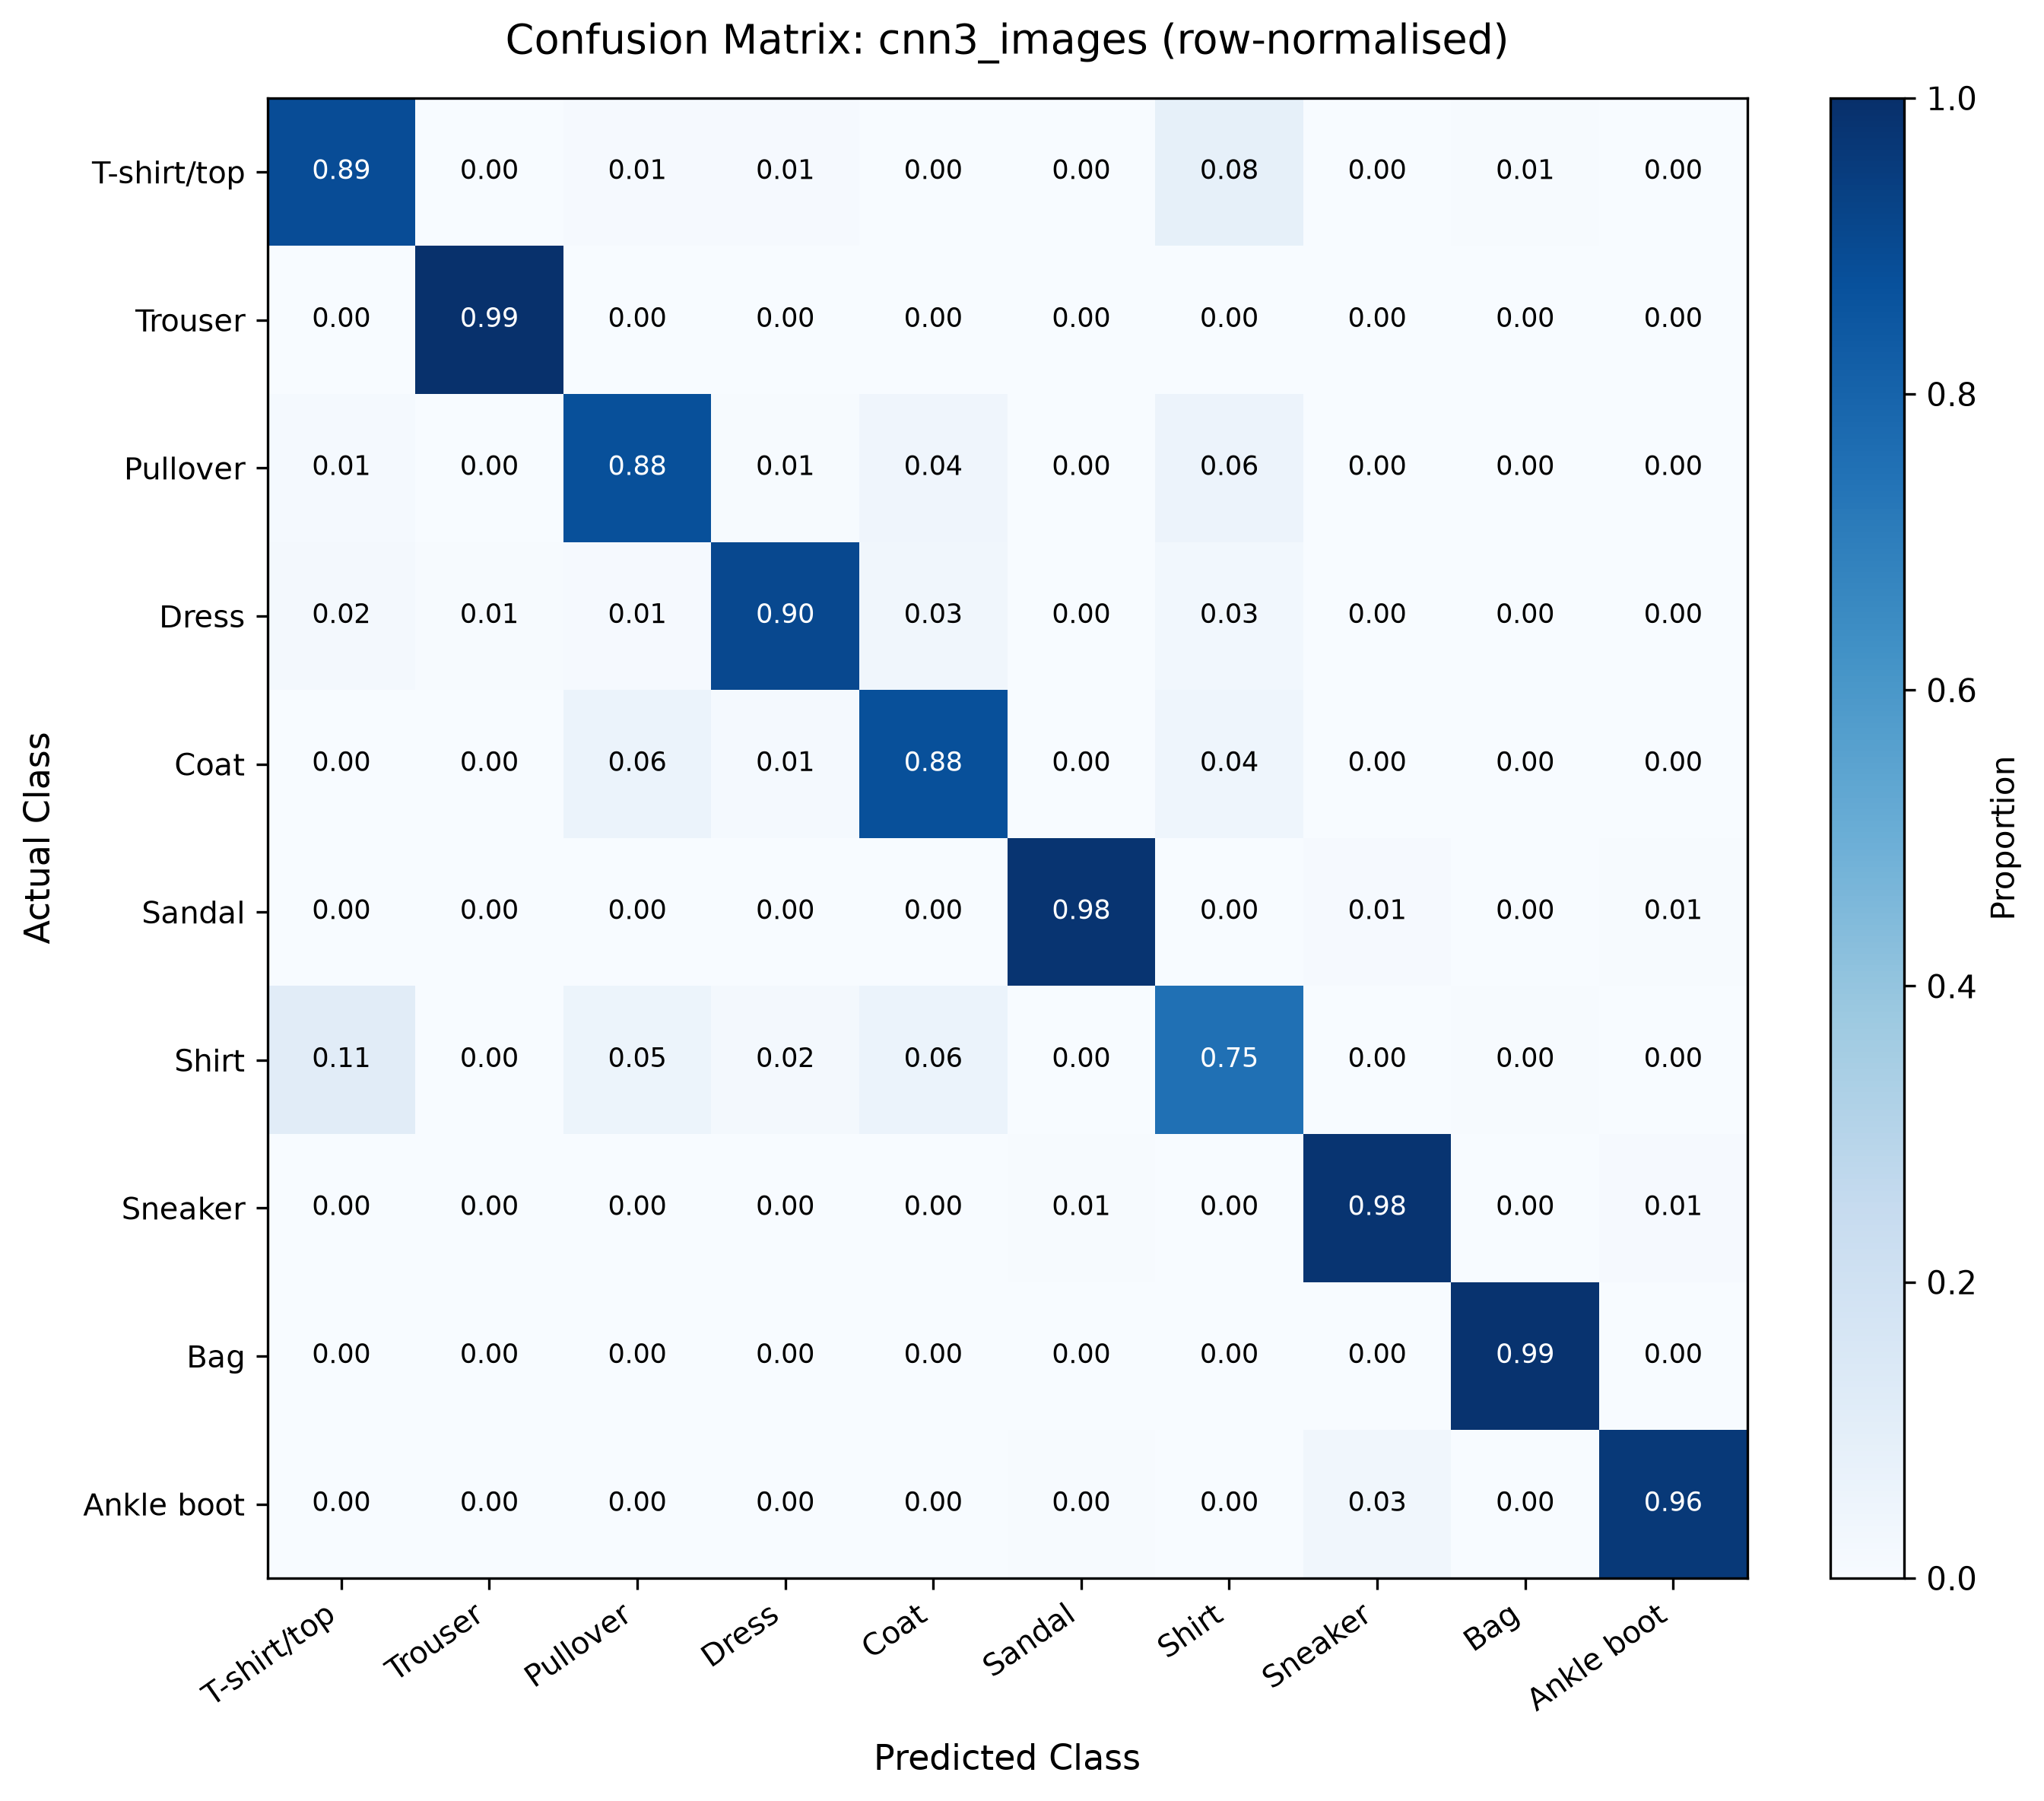
\includegraphics[width=0.92\linewidth]{errors_confusion_cnn3_images.png}
  \caption{Row-normalized test confusion matrix of CNN3. The upper-body garments still form the dominant off-diagonal
  block, as they did for every classical model.}
  \label{fig:cm}
\end{figure}

\begin{table}[t]
  \centering
  \caption{Agreement of CNN3 and the RBF SVM (HOG) on the Test Set}
  \label{tab:agree}
  \resizebox{\columnwidth}{!}{%
  \begin{tabular}{@{}l c c r@{}}
    \toprule
    & \multicolumn{2}{c}{RBF SVM / HOG} & \\
    \cmidrule(lr){2-3}
    CNN3 & correct & wrong & Total \\
    \midrule
    correct & 8{,}792 & 417 & 9{,}209 \\
    wrong   & 316     & 475 & 791 \\
    \midrule
    Total   & 9{,}108 & 892 & 10{,}000 \\
    \bottomrule
  \end{tabular}}
\end{table}

\textbf{Shared errors point to the data.} The two models share no features---one sees gradient histograms through a
kernel, the other learned filters---yet of the 475 images both misclassify, 398 (83.8\%) receive \emph{the same} wrong
label and 362 (76.2\%) are upper-body garments. \Cref{fig:mis} shows the first eight test shirts, in test order and not
hand-picked, that each model calls T-shirt/top: most are short-sleeved and collarless, and two (test \#612 and \#1129) are
sleeveless tank tops. At the level of single images the trade is visible: CNN3 correctly identifies test \#40, whose
button placket is visible, which the SVM misses, while the SVM correctly classifies \#612 and \#1129, which CNN3 misses.

\begin{figure}[t]
  \centering
  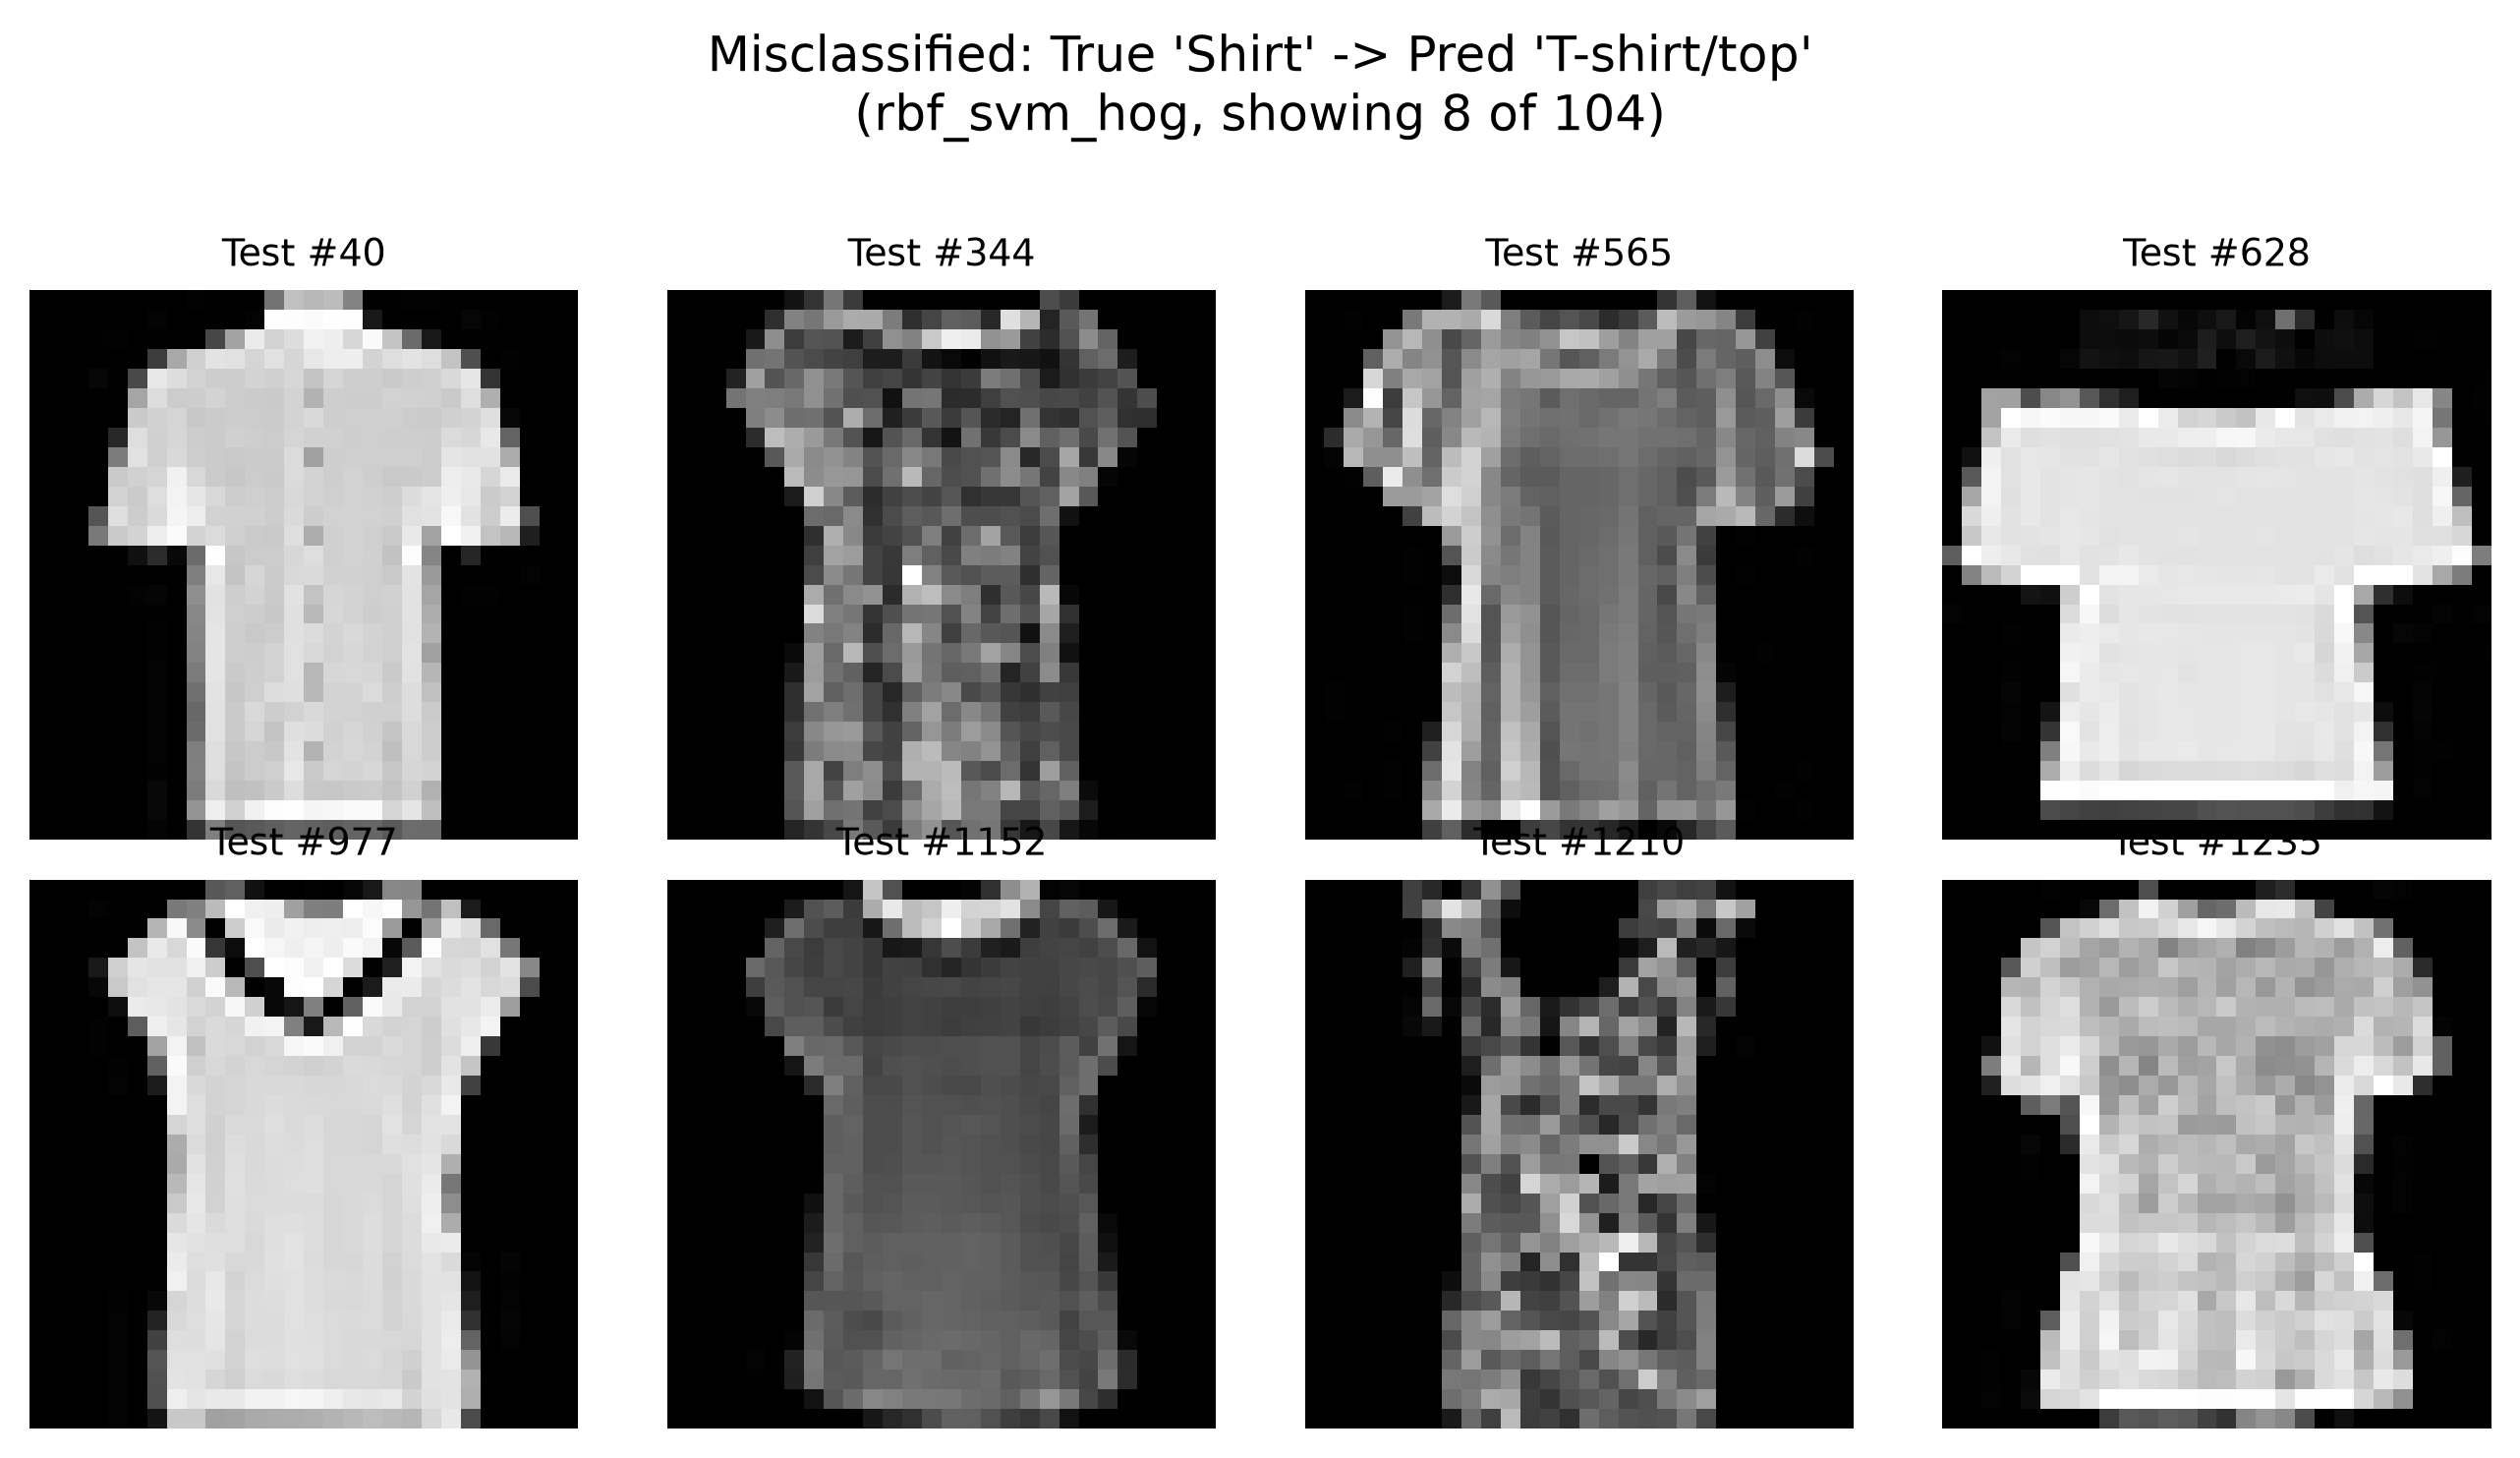
\includegraphics[width=\linewidth]{errors_misclassified_rbf_svm_hog_shirt_vs_t-shirt_top.png}\\[4pt]
  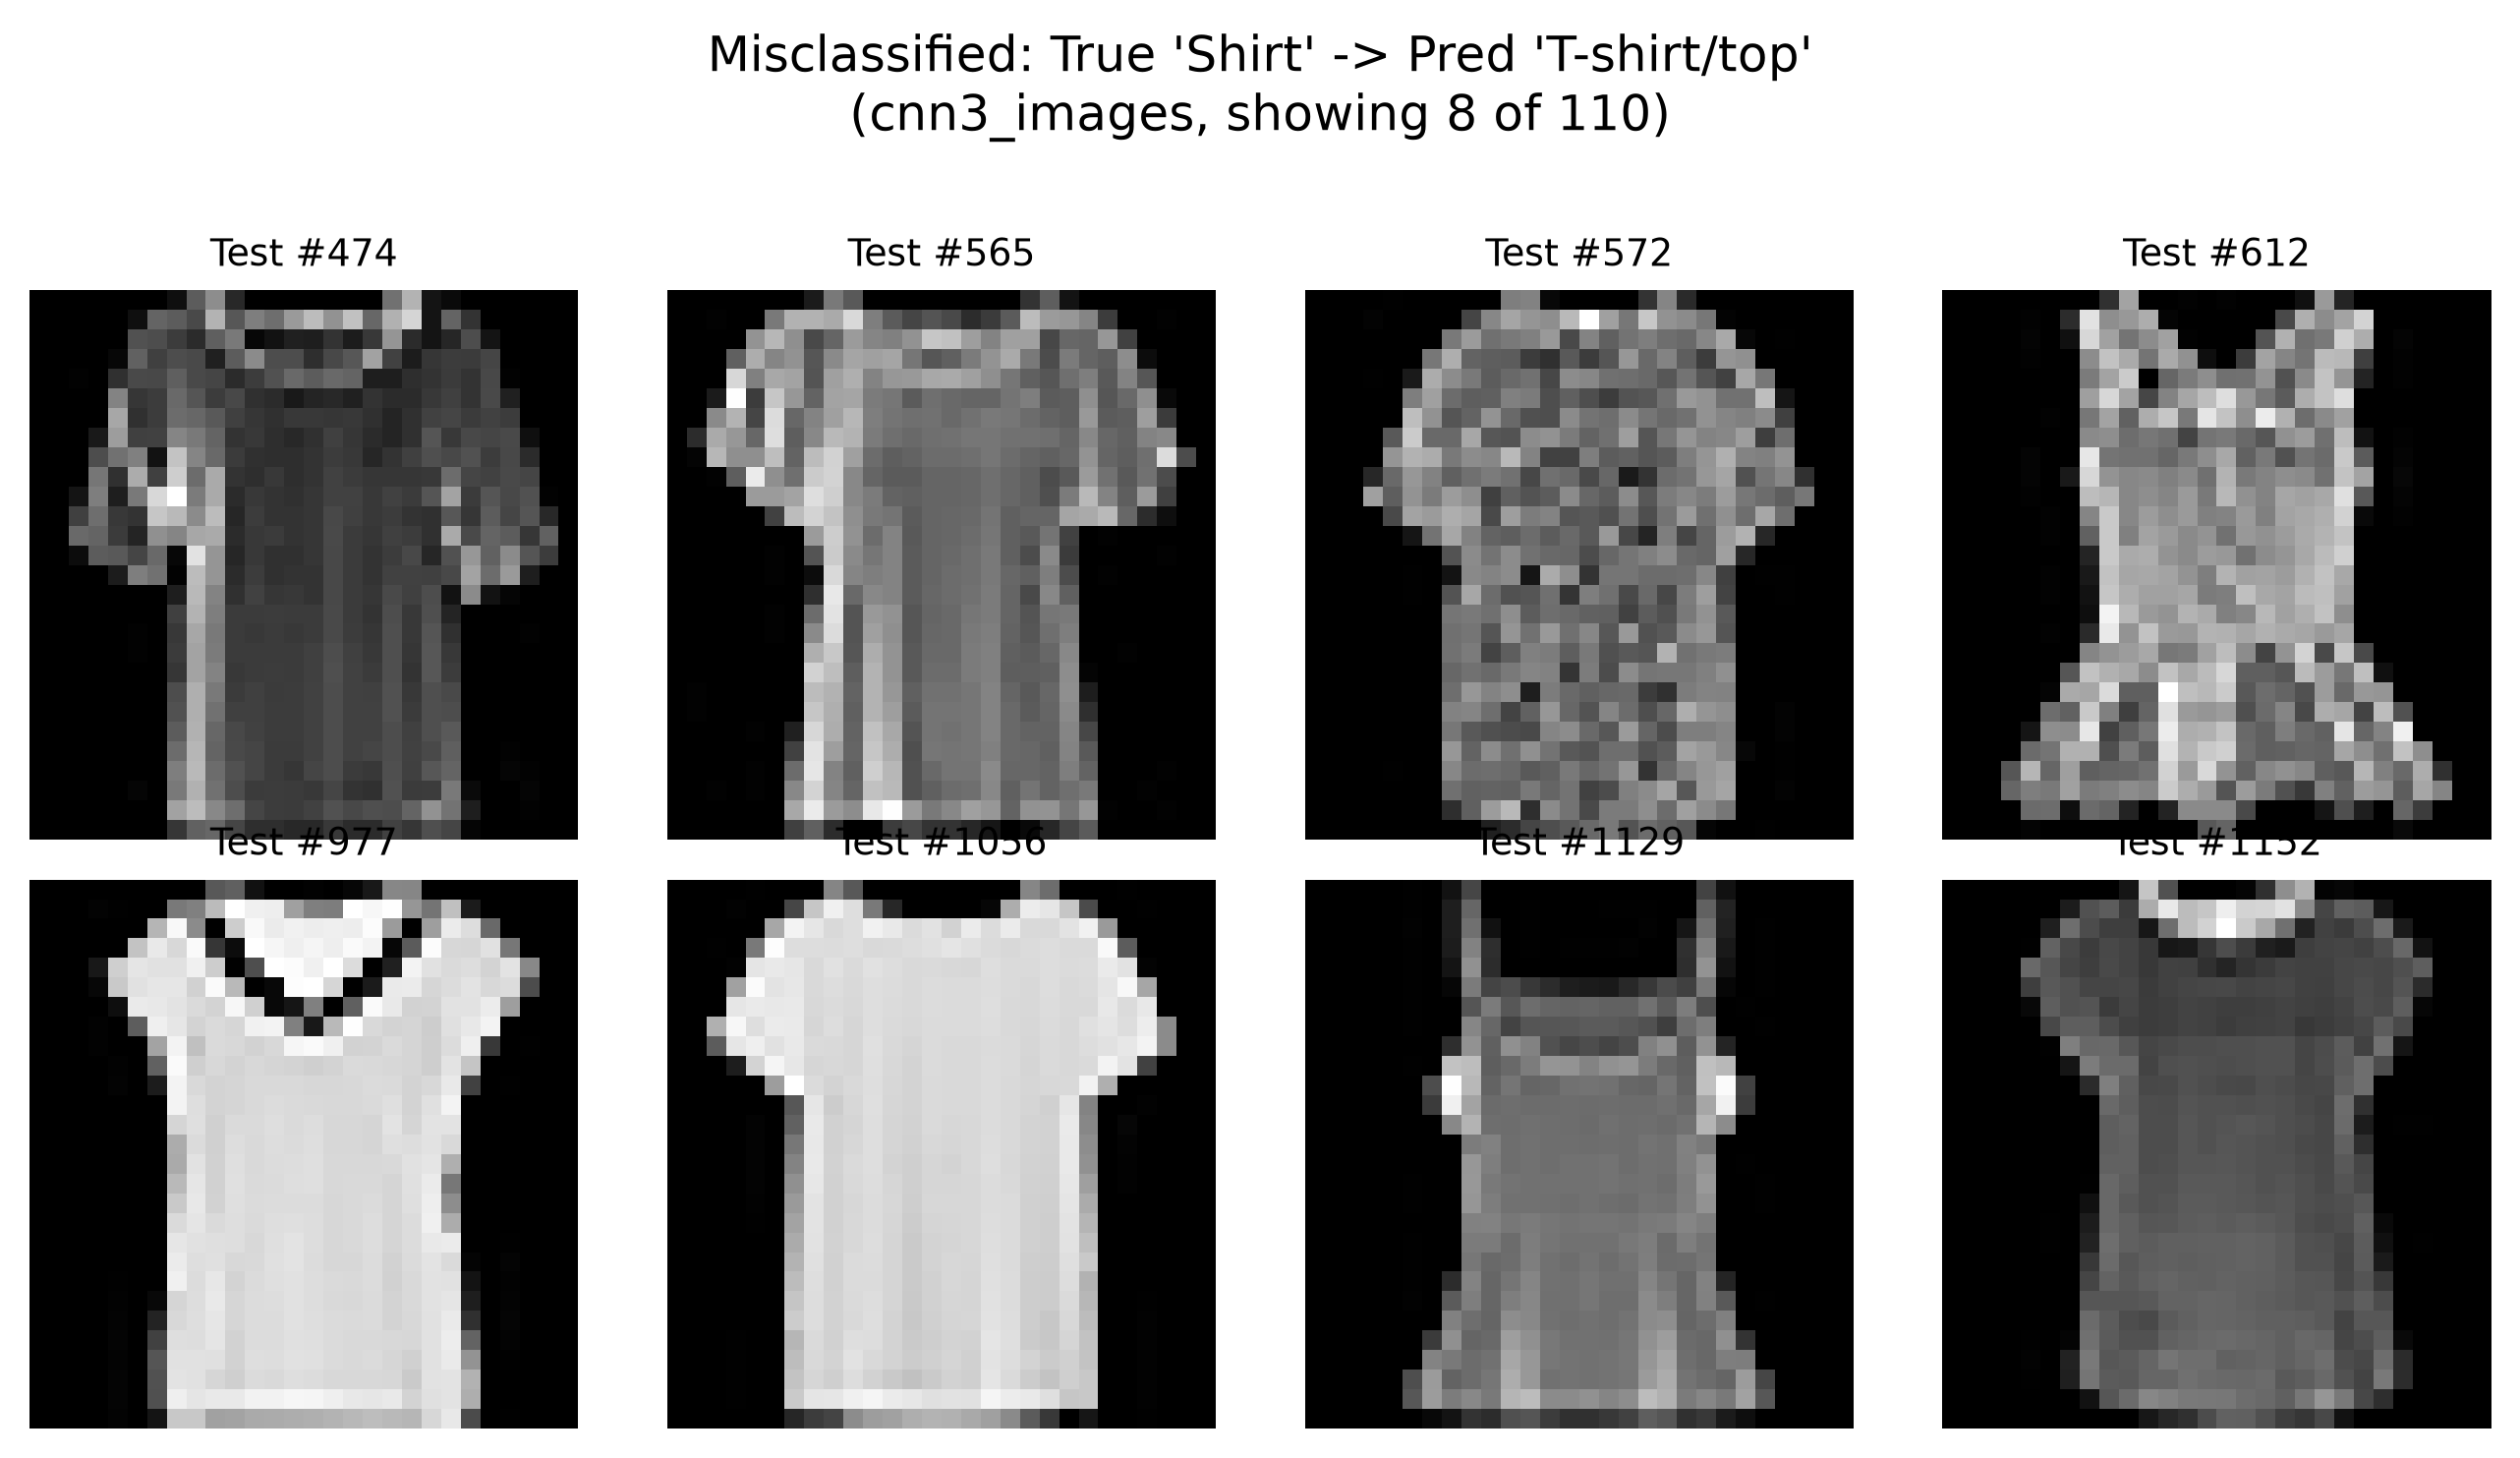
\includegraphics[width=\linewidth]{errors_misclassified_cnn3_images_shirt_vs_t-shirt_top.png}
  \caption{The first eight test images of class Shirt predicted as T-shirt/top by the RBF SVM on HOG (top, 8 of 104) and
  by CNN3 (bottom, 8 of 110). Several are collarless or sleeveless garments whose label is ambiguous at this resolution.}
  \label{fig:mis}
\end{figure}

% =====================================================================================
\section{Hybrid: Learned Features, Classical Classifier}
\label{sec:hybrid}

\subsection{Motivation and Method}
CNN3 differs from the RBF SVM on HOG in \emph{two} ways: its features are learned instead of fixed, and its classifier is
a softmax layer instead of a kernel machine. A gain could come from either. Agarap~\cite{agarap2017cnnsvm} swapped the
classifier but retrained the network with it, so features and classifier changed together; we instead freeze the
features and swap only the classifier. Writing CNN3 as $f=h_{\text{soft}}\circ\phi$,
with
\begin{equation}
  \begin{gathered}
  \phi(\mathbf{x}) = \max\!\big(0,\; W_1\,\mathrm{vec}(g(\mathbf{x}))+\mathbf{b}_1\big)\in\mathbb{R}^{128}_{\ge 0},\\
  h_{\text{soft}}(\mathbf{z}) = \argmax_k\,(W_2\mathbf{z}+\mathbf{b}_2)_k ,
  \end{gathered}
  \label{eq:phi}
\end{equation}
where $g$ denotes the three conv blocks, we build the \hyb{} $f'=h_{\text{RBF}}\circ\phi$: the \emph{frozen} CNN3
representation followed by the Phase~1 RBF SVM. The two one-component swaps then isolate each factor:
\begin{itemize}
  \item \textbf{same classifier, different features:} RBF SVM on HOG vs.\ \hyb{};
  \item \textbf{same features, different classifier:} CNN3 vs.\ \hyb{}.
\end{itemize}
CNN3's weights are not updated: they were learned from the 54k training split only, and extracting $\phi$ fits nothing,
so $\phi$ is a fixed feature map like HOG. The protocol, committed before the run, is exactly Phase~1's RBF SVM track: the
same $3\times3$ grid on a stratified 10k subset, a 54k refit scored on validation, a 60k refit and one test evaluation. As
a check that the right layer is tapped, CNN3's own output layer applied to the extracted validation features reproduces
CNN3's validation accuracy, 0.9308.

Two properties of $\phi$ matter. First, it is sparse: 77.5\% of the activations are zero, and 47 of the 128 units are
zero for \emph{every} training and validation image (dead ReLUs), so the representation is effectively 81-dimensional.
After standardization the overall variance of the feature matrix is therefore $81/128$, and $\gamma=\texttt{scale}$
evaluates to $1/81\approx0.0123$. Second, it is compact: 128 dimensions against HOG's 1{,}728, which makes every
kernel evaluation over $13\times$ cheaper.

\subsection{Results (RQ9)}
Every grid point fits the 10k subset in under 1.5\,s and scores 0.9148--0.9292 on validation; $C=1$,
$\gamma=\texttt{scale}$ is selected. Refit on 54k it scores \textbf{0.9313}, tied with CNN3 (0.9308) and well above the
SVM on HOG (0.9157). On test, the \hyb{} reaches \textbf{92.44\%} (95\% CI 91.91--92.94\%) and macro-F1 \textbf{0.9241},
with 756 errors---the best result of all 15 experiments (\cref{tab:results}).

\textbf{Decomposition.} \Cref{tab:decomp} lists the two paired comparisons. Holding the classifier fixed, learned
features add $+1.36$\pp{} over HOG (430 vs.\ 294 images; $\chi^2=25.2$, $p=5.2\times10^{-7}$). Holding the features fixed,
the SVM adds $+0.35$\pp{} over the softmax layer (110 vs.\ 75 images; $\chi^2=6.25$, $p=0.012$). The representation
accounts for roughly four times as much accuracy as the classifier. Moreover, the classifier effect is not visible on
validation (0.9313 vs.\ 0.9308) and is partly confounded: the \hyb{}'s SVM was refit on 60k images while CNN3's output
layer learned from 54k. We therefore read it as small and uncertain, and the representation effect as the robust
finding: \emph{what moved Phase~2 past Phase~1 is what the network learned to see, not how it decides.}

\begin{table}[t]
  \centering
  \caption{Feature--Classifier Decomposition (Paired Test Comparisons)}
  \label{tab:decomp}
  \setlength{\tabcolsep}{3pt}
  \resizebox{\columnwidth}{!}{%
  \begin{tabular}{@{}l l r c c@{}}
    \toprule
    Swap (A vs.\ B) & Held fixed & $\Delta$acc & only A / only B & $p$ \\
    \midrule
    \hyb{} vs.\ RBF/HOG & classifier & $+1.36$\pp & 430 / 294 & $5.2{\times}10^{-7}$ \\
    \hyb{} vs.\ CNN3    & features   & $+0.35$\pp & 110 / 75  & $0.012$ \\
    CNN3 vs.\ RBF/HOG   & neither    & $+1.01$\pp & 417 / 316 & $2.2{\times}10^{-4}$ \\
    \bottomrule
  \end{tabular}}\\[2pt]
  {\footnotesize only A / only B: test images classified correctly by one model only. $p$: McNemar, \cref{eq:mcnemar}.}
\end{table}

\textbf{Shirt is still not fixed.} The \hyb{}'s Shirt recall is 73.8\%, below both CNN3 (75.1\%) and the SVM (75.2\%);
Shirt\arrowc T-shirt/top rises to 117. Its gains over CNN3 are on Dress ($+2.5$\pp) and Coat ($+1.5$\pp)
(\cref{fig:hybrid}), and confusions among the four tops now make up 521 of its 756 errors (68.9\%), the highest share of
any model. The \hyb{} and CNN3 share 681 errors, and on 659 of them (96.8\%) they choose the same wrong label: a different
decision rule on the same features makes almost exactly the same mistakes. This is the strongest evidence in the study
that the residual error lives in the images.

\begin{figure*}[t]
  \centering
  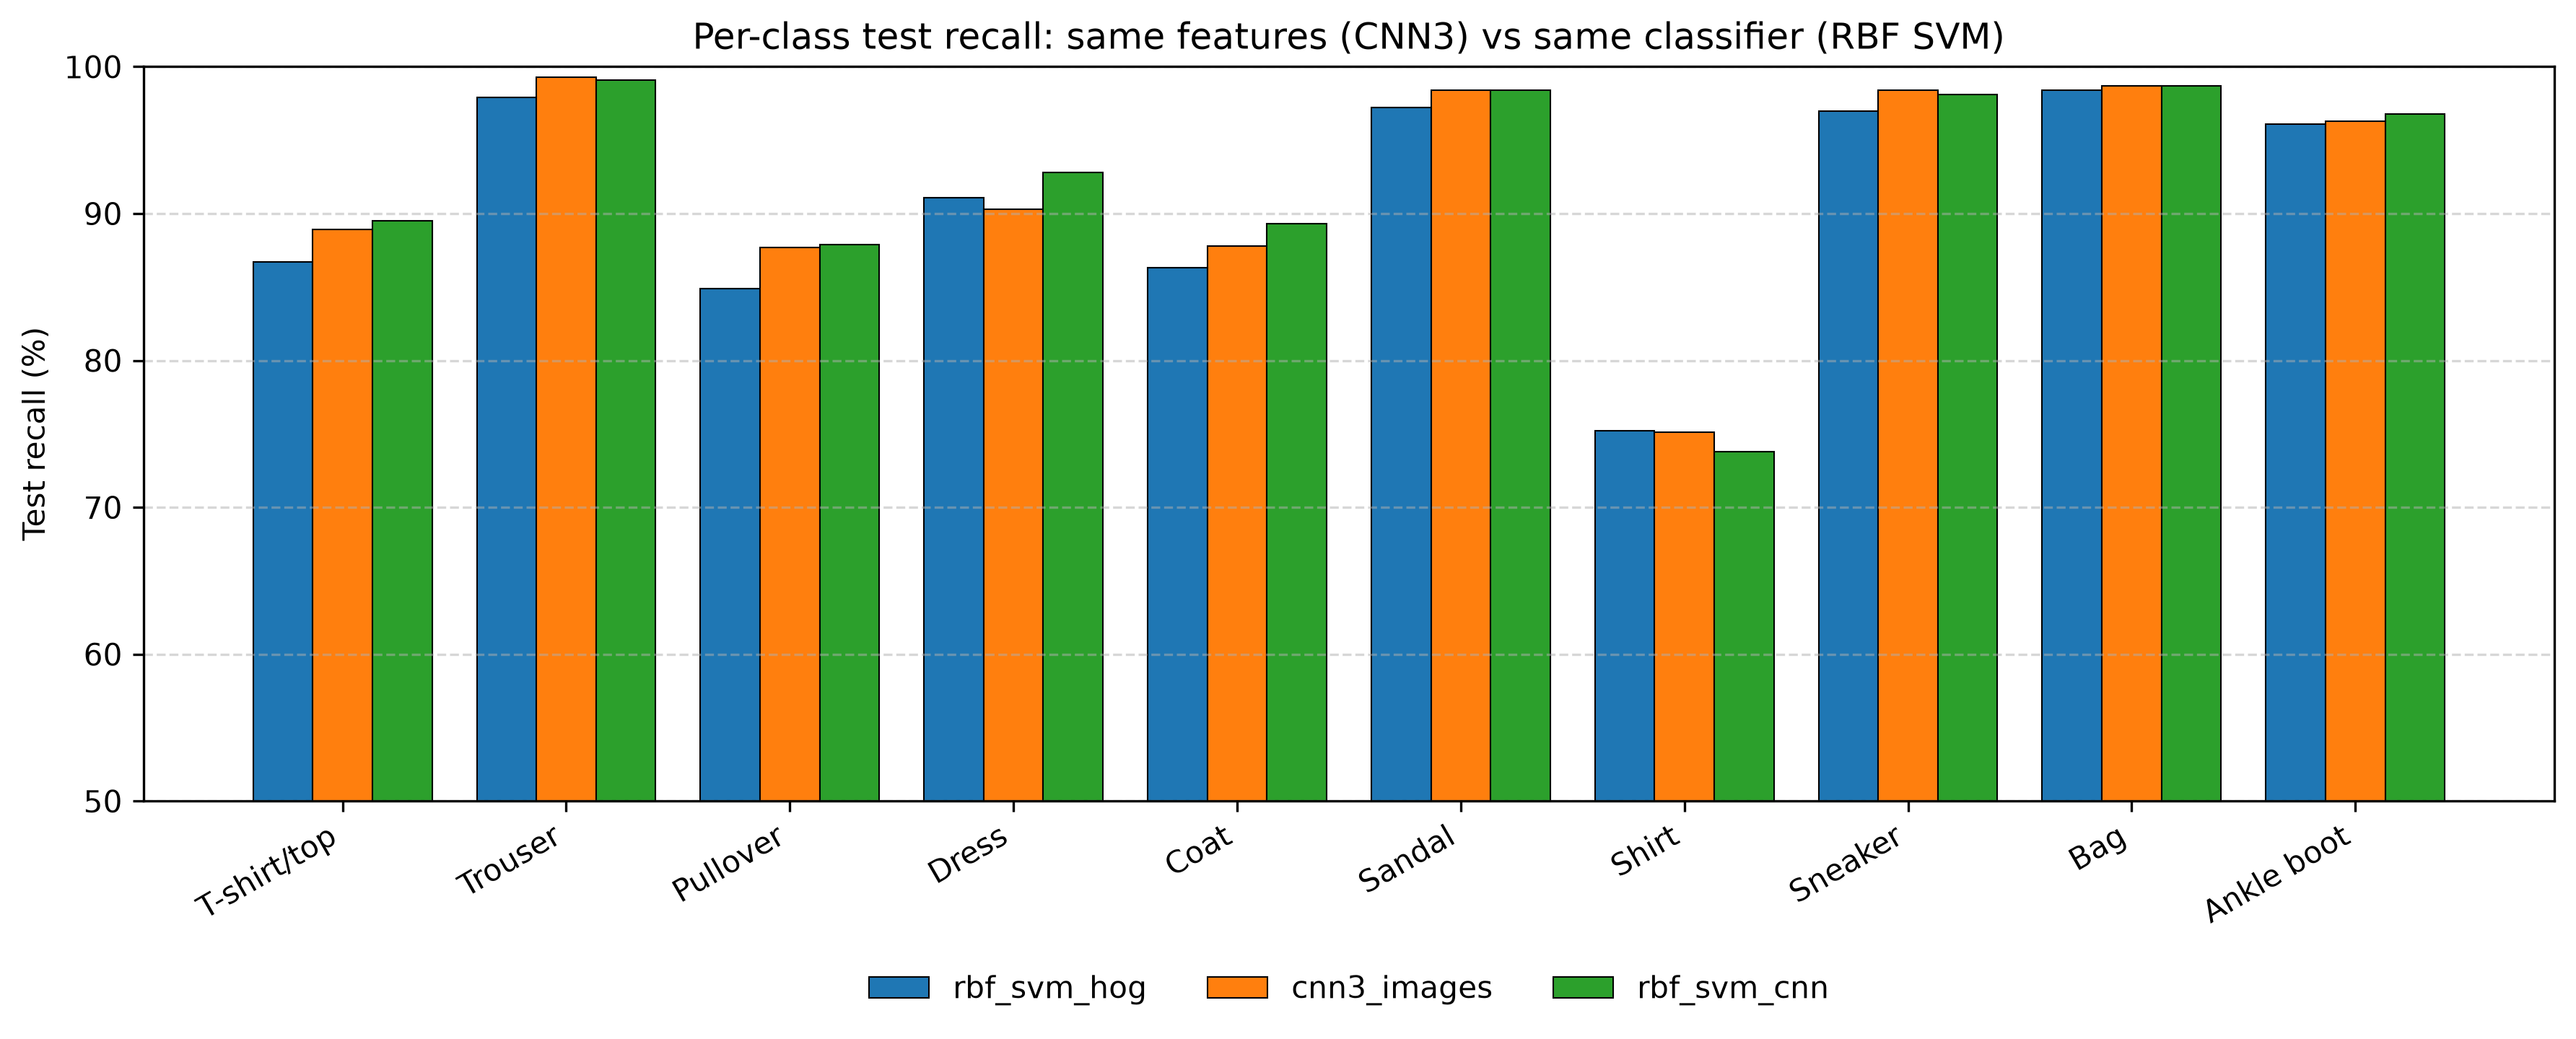
\includegraphics[width=0.9\linewidth]{hybrid_recall_vs_cnn3.png}
  \caption{Per-class test recall of the RBF SVM on HOG, CNN3 and the \hyb{}. Learned features lift almost every class;
  no representation or classifier lifts Shirt.}
  \label{fig:hybrid}
\end{figure*}

\textbf{Cost.} The \hyb{}'s SVM keeps 7{,}919 support vectors of dimension 128, against 26{,}343 of dimension 1{,}728 for
the SVM on HOG, so it predicts ${\sim}59\times$ faster on precomputed features (491\,ms vs.\ 28{,}877\,ms per 1{,}000
images). End to end, including 118\,ms of CNN3 feature extraction, it needs ${\approx}609$\,ms, ${\sim}48\times$ faster
than the SVM on HOG but ${\sim}6.5\times$ slower than CNN3 alone, from a ${\approx}9.7$\,MB model (8.7\,MB of support
vectors plus CNN3's layers), ten times CNN3's size. For deployment, 0.35\pp{} does not justify that cost.

% =====================================================================================
\section{Discussion}
\label{sec:discussion}
\textbf{Why did H2 fail?} H2 assumed the Shirt confusion was a \emph{representation} problem---that the discriminative
detail was in the image and HOG failed to encode it. Four observations argue instead for an \emph{information} problem.
(i)~Two representations with nothing in common fail on largely the same images with the same wrong label. (ii)~The CNN's
improvement is broad, spanning footwear, trousers and the other tops, which is what a generally better feature extractor
produces; a targeted fix would have concentrated on Shirt. (iii)~Changing the classifier on top of the learned features
moves Dress and Coat but not Shirt, and repeats 96.8\% of the shared wrong labels. (iv)~The failures include collarless
and sleeveless garments that a human annotator could reasonably label either way. More capacity, augmentation or data can
sharpen decision boundaries but cannot recover a collar two pixels wide or resolve a genuinely ambiguous label. We
therefore read 92\% not as a modest CNN result but as evidence that much of the remaining error may lie close to the limit set
by the data. This is an inference from shared errors, not a measured ceiling; Future work~(iii) proposes the test.

\textbf{Representation over classifier.} The decomposition gives a direct answer to the question behind the project:
the same kernel machine is 1.36\pp{} better on learned features than on the best handcrafted ones, while the choice
between kernel machine and softmax layer is worth about a third of a point, which may be within seed variation.

\textbf{Relation to the earlier CNN--SVM result.} Agarap~\cite{agarap2017cnnsvm} found an SVM output layer
1.14\pp{} \emph{worse} than softmax on Fashion-MNIST; we find an SVM on frozen features 0.35\pp{} \emph{better}. The two
findings are compatible. There the SVM was linear and trained jointly with the network, so its features differed too;
here it is a kernel machine on fixed features. In both studies the effect of the classifier is about one point or less,
and its sign depends on how the classifier is attached---whereas the effect of the representation, measured with the
classifier held fixed, is larger and highly significant. Independently, that study's two-layer CNN with softmax reached
91.86\%, within 0.01\pp{} of our two-block CNN2 (91.85\%) under a different training protocol, which suggests that our
CNN results are typical of networks of this size rather than an artifact of our setup.

\textbf{Which model to deploy?} For catalog tagging, CNN3: within 0.35\pp{} of the most accurate model, about 0.1\,s per
1{,}000 images, and under 1\,MB. Among classical models, the 181\,KB Linear SVM on HOG remains the practical choice
(88.98\%, ${\approx}219$\,ms per 1{,}000 images); CNN3 adds three points at less than half that time.

\textbf{Threats to validity.}
\begin{itemize}
  \item \textbf{One training run per network.} Seed variance was not measured systematically; the one repetition
        (CNN2: 0.9228 vs.\ 0.9320 on validation) suggests about 1\pp. The CNN-vs-SVM and features-vs-HOG conclusions rest
        on paired tests over 10{,}000 images; CNN3-vs-CNN2 is explicitly inconclusive, and the 0.35\pp{} classifier effect
        may lie within seed variation.
  \item \textbf{Unequal training data.} CNNs saw 54k images; classical models and the \hyb{}'s SVM saw 60k. This biases
        the CNN comparisons against the CNN and the classifier comparison in favor of the \hyb{}.
  \item \textbf{Fixed hyperparameters.} No learning-rate, width or dropout search was run, and three classical models
        selected a value on the edge of their grid; all results are lower bounds for their model families.
  \item \textbf{Optimistic validation.} Validation exceeds test accuracy for every trained model (by 0.02--2.05\pp), the
        selection bias expected when choosing the best of several settings on validation; we report test scores.
  \item \textbf{Timing hardware.} Timings come from an Apple M3 and an M3 Pro; only order-of-magnitude gaps are firm.
  \item \textbf{Label quality.} Our evidence of ambiguous labels is qualitative; no image was relabeled.
\end{itemize}

% =====================================================================================
\section{Conclusion and Future Work}
\label{sec:conclusion}
Under one protocol that holds the split, the test set and the evaluation code fixed across 15 experiments, a carefully
tuned classical pipeline reaches 91.08\% on Fashion-MNIST; a three-block CNN with fewer than a quarter of a million
parameters reaches 92.09\% at ${\sim}1/300$ of the prediction time and ${\sim}1/377$ of the size; and the RBF SVM trained on
the CNN's own features reaches 92.44\%. The CNN wins (H1), but not by fixing the shirts (H2): the gain is broad, comes
mostly from the learned representation rather than the classifier, and stops at a residual error that models
with entirely different views of the image share, label for label. The evidence points to the resolution and labeling of
the data, rather than the choice between handcrafted and learned features, as the binding constraint; we have not tested
this directly. Read together with the original benchmark~\cite{xiao2017fashion}, our Phase~1 study~\cite{phase1report}
and the earlier CNN--SVM comparison~\cite{agarap2017cnnsvm}, the results give a consistent picture: careful protocol
moves classical models by about a point, learned features by about another, and the choice of classifier by less.

\textbf{Future work.} (i)~Train over several seeds to bound variance and settle the depth and classifier comparisons.
(ii)~Refit the \hyb{}'s SVM on 54k images to remove the training-data confound. (iii)~Audit the shared errors with
a relabeling study to estimate how much residual error is label noise. (iv)~Test whether
augmentation or higher-resolution inputs move Shirt recall, which would distinguish a capacity limit from an information
limit.

\textbf{Reproducibility.} Code, the committed split, all result files, training histories, figures, the test-set audit
log and a decision log recording the reason for every choice are available at
\url{https://github.com/rajdeep-2004/fashion-image-classification-benchmark}. Training is seeded and deterministic on CPU;
a fresh clone runs all eight notebooks in about two minutes and regenerates every reported number.

% =====================================================================================
\begin{thebibliography}{3}

\bibitem{xiao2017fashion}
H.~Xiao, K.~Rasul, and R.~Vollgraf, ``Fashion-MNIST: A novel image dataset for benchmarking machine learning
algorithms,'' \emph{arXiv preprint arXiv:1708.07747}, 2017.

\bibitem{phase1report}
T.~Singh, A.~Mishra, R.~Sanyal, R.~Srivastav, and O.~Nagre, ``How far can classical machine learning go on
Fashion-MNIST? A leak-free benchmark of raw pixels vs.\ HOG features, with cost and error analysis,'' Capstone Project
Report (Phase~1), Newton School of Technology, Rishihood University, 2026.

\bibitem{agarap2017cnnsvm}
A.~F.~Agarap, ``An architecture combining convolutional neural network (CNN) and support vector machine (SVM) for
image classification,'' \emph{arXiv preprint arXiv:1712.03541}, 2017.

\end{thebibliography}

\end{document}
